% !TEX root = ../thesis-example.tex
%
\chapter{Notions et éléments de la géométrie classique et de la géométrie digitale}
\label{sec:notions}

% \cleanchapterquote{We have seen that computer programming is an art, because it applies accumulated knowledge to the world, because it requires skill and ingenuity, and especially because it produces objects of beauty.}{Jean-Claude Vandamme}{Ma vie, mon œuvre.}

\setcounter{minitocdepth}{3}
\minitoc

\newpage
%
\section{Introduction}
%
Dans ce chapitre, nous allons poser les définitions des éléments dont nous
allons nous servir pour la suite de ce document. Cela comprend une introduction à
la géométrie des surfaces et des formes continues (\RefSectionN{sec:geo-diff}) permettant
de faire le lien entre la géométrie euclidienne et nos estimateurs digitaux, les
notions de base de la géométrie digitale (\RefSectionN{sec:notions-base}), ainsi
que tout le processus formel permettant d'analyser le comportement d'un estimateur
digital (\RefSectionN{sec:multigrid-convergence-estimator}). Enfin, nous verrons
quelques primitives digitales que nous utiliserons par la suite, comme les
segments de droite discrète maximaux (\RefSectionsN{sec:aire-volume-moments}{sec:segments}).
% historique geo dis : http://www.citr.auckland.ac.nz/~rklette/talks/01_CP.pdf
%
\section{Notations}
%
Le \RefTable{tab:notations} énonce les notations utilisées dans ce manuscrit et
leur signification (sauf mention contraire). Chacune de ces notations sera
introduite au cours des différents paragraphes.

\begin{table}[ht]
  \centering
  \caption{Notations utilisées dans cette thèse}
  \label{tab:notations}
    \renewcommand{\arraystretch}{1.1}
  \begin{tabular}{@{}lp{9cm}r@{}}
    \toprule
    Notation      & Description  & Définition \\ \midrule

    $\R^d$        & Espace euclidien de dimension $d$ & \\%\RefSectionTable{sec:notions} \\
    $\Shapes$     & Famille de formes convexes de $\R^d$ de bord $C^3$ à courbure bornée & \RefSectionTable{sec:multigrid-convergence-estimator} \\
    $\Shape$      & Forme de $\Shapes$ & \RefSectionTable{sec:multigrid-convergence-estimator} \\
    $\dS$         & Bord topologique de $\Shape$ & \RefSectionTable{sec:digitization} \\
    $\vx$         & Point de $\R^d$ & \RefSectionTable{sec:digitization} \\
    $x_i$         & $i$-ième coordonnée de $\vx$ avec $\vx=(x_1, \ldots, x_d)$ & \\%\RefSectionTable{sec:notions} \\
    $\vx_i$       & $(i+1)$-ième point d'une séquence. $(\vx_i)_{i=0 \cdots n-1}$ & \\%\RefSectionTable{sec:notions} \\
    $\Z^d$        & Espace en coordonnées entières de dimension $d$ & \RefSectionTable{sec:digitization} \\
    $\DigShape$   & Objet digital (partie de $\Z^d$) & \RefSectionTable{sec:digitization} \\
    $h$           & Pas de discrétisation pour la discrétisation de Gauss & \RefSectionTable{sec:digitization} \\
    $\DSh$        & Discrétisation de Gauss de $\Shape$ sur une grille de pas $h$ & \RefSectionTable{sec:digitization} \\
    $\Body{\DSh}{h}$ & Plongement euclidien de la discrétisation de Gauss de $\Shape$ sur une grille de pas $h$ & \RefSectionTable{sec:digitization} \\
    $\partial\Body{\DSh}{h}$ & Bord topologique du plongement euclidien de la discrétisation de Gauss de $\Shape$ sur une grille de pas $h$ & \RefSectionTable{sec:digitization}\\
    $\hat{\vx}$   & Points de $\partial\Body{\DigShape}{h}$ pour une forme $\DigShape$ & \RefSectionTable{sec:digitization} \\


    $E(\Shape,\vx)$                   & Quantité définie au point $\vx \in \dS$, $\Shape \subset \R^d$ & \RefSectionTable{sec:multigrid-convergence-estimator} \\
    $\hat{E}(\DigShape,\hat{\vx},h)$  & Quantité estimée au point $\hat{\vx} \in \partial\Body{\DigShape}{h}$, $\DigShape \subset \Z^d$ & \RefSectionTable{sec:multigrid-convergence-estimator} \\
    $\Mom{p_1 \cdots p_d}(\Shape)$    & Moment géométrique d'ordre $p_1 \cdots p_d$ de $\Shape$ & \RefSectionTable{sec:moments-geo} \\
    $\Cov(\Shape)$                    & Matrice de covariance de $\Shape$ & \RefSectionTable{sec:pottmann-principle} \\
    $\Curv(\Shape,\vx)$               & Courbure au point $\vx \in \dS$, $\Shape \subset \R^2$ & \RefSectionTable{sec:geo-diff} \\
    $\MeanCurv(\Shape,\vx)$           & Courbure moyenne au point $\vx \in \dS$, $\Shape \subset \R^3$ & \RefSectionTable{sec:geo-diff} \\
    $\GaussCurv(\Shape,\vx)$          & Courbure gaussienne au point $\vx \in \dS$, $\Shape \subset \R^3$ & \RefSectionTable{sec:geo-diff} \\
    $\PrincCurv{i}(\Shape,\vx)$       & $i$-ième courbure principale au point $\vx \in \dS$, $\Shape \subset \R^3$ & \RefSectionTable{sec:geo-diff} \\
    $\PrincDir{i}(\Shape,\vx)$        & $i$-ième direction principale de courbure au point $\vx \in \dS$, $\Shape \subset \R^3$ & \RefSectionTable{sec:geo-diff} \\
    $\NormalDir(\Shape,\vx)$          & Normale au point $\vx \in \dS$, $\Shape \subset \R^3$ & \RefSectionTable{sec:geo-diff} \\
    \bottomrule
  \end{tabular}
\end{table}
%
\section{Introduction à la géométrie des surfaces et formes continues}
\label{sec:geo-diff}
%
La \colorize{géométrie des surfaces et des formes continues} est l'étude des
surfaces comme graphes de fonctions. Nous allons dans un premier temps étudier
la dérivabilité de ces fonctions (\colorize{classes de fonctions}). Ensuite,
nous définirons des quantités intégrales décrivant la surface.


%
% Introduction à la géométrie différentielle ?
%
% courbure : Defining and studying the curvatures of singular spaces goes back to Steiner (1840) in the convex case (see [30] for instance). ([30] = L. Santalo, Integral geometry anf geometric probability, Encyclopedia of Math- ematics and its applications, Vol. 1. Addison-Wesley Publishing Co. (1976), MR0433364, Zbl 0342.53049.)

\subsection{Classes de fonctions $C^1$, $C^2$, $C^d$}
%
Définissons les classes de fonctions $C^1$, $C^2$ ou plus généralement
$C^d$, permettant de connaître le différentiabilité d'une fonction.
%
\begin{definition}{\fakeTitle{Classe de fonction $C^1$}}
  %
  Une fonction $f$ sur un intervalle réel non vide et non trivial est une
  fonction continûment différentiable si elle est différentiable et si sa
  dérivée $f'$ est continue. Nous dirons également que $f$ est de
  \colorize{classe $C^1$}.
  %
\end{definition}
%
\begin{definition}{\fakeTitle{Classe de fonction $C^2$}}
  %
  Une fonction $f$ sur un intervalle réel non vide et non trivial est une
  fonction deux fois continûment différentiable si elle est deux fois
  différentiable et si sa dérivée seconde $f''$ (la dérivée de $f'$) est
  continue. Nous dirons également que $f$ est de \colorize{classe $C^2$}.
  %
\end{definition}
%
Plus généralement, pour $d>2$, la classe de fonction $C^d$ est définie comme :
%
\begin{definition}{\fakeTitle{Classe de fonction $C^d$}}
  %
  Une fonction $f$ est de \colorize{classe $C^d$} (avec $d \ge 2$) sur un
  intervalle réel non vide et non trivial si elle est $d$ fois continûment
  différentiable.
  %
\end{definition}
%
\subsection{Aire et volume}
%
Nous nous intéressons aux quantités intégrales d'une forme $\Shape \subset
\R^d$. Les quantités les plus directes sont probablement l'aire de la forme en
dimension 2 ou son volume en dimension 3. Cela revient à calculer une double ou
triple intégrale de la forme suivante :
%
\begin{definition}{\fakeTitle{Aire d'une forme}}
  %
  Soit $\Shape$ une partie bornée de $\R^2$. Soit la fonction constante $1$
  intégrable sur $\Shape$, alors \colorize{l'aire} de $\Shape$ est :
  %
  \begin{equation}
    \label{eq:aire}
    \Area(\Shape) = \iint_{\Shape} dxdy \,.
  \end{equation}
  %
\end{definition}
%
\begin{definition}{\fakeTitle{Volume d'une forme}}
  %
  Soit $\Shape$ une partie bornée de $\R^3$. Soit la fonction constante $1$
  intégrable sur $\Shape$, alors \colorize{le volume} de $\Shape$ est :
  %
  \begin{equation}
    \label{eq:volume}
    \Vol(\Shape) = \iiint_{\Shape} dxdydz \,.
  \end{equation}
  %
\end{definition}
%
Nous parlons également de mesure de $\Shape$ au sens de Lebesgue. Nous
reviendrons sur ces définitions dans le cadre digital dans le \RefSection{sec:aire-volume-moments}.
%
\subsection{Moments géométriques}
\label{sec:moments-geo}
%
Le concept mathématique des moments (\anglais{General moment theory}) a été
activement étudié depuis plusieurs années. Plus particulièrement, les moments
géométriques ont montré leur intérêt dans la reconnaissance de formes (nous
pouvons citer la revue de \cauthors{Trier}{Trier1996} pour la reconnaissance de
caractères) et la reconstruction d'objets \cite{Ghorbel2005}. La première
utilisation des moments en analyse d'images remonte à 1962 par
\cauthor{Hu}{Hu1962} pour la reconnaissance de caractères.
%
% Les moments ont l'avantage d'être indépendant à l'échelle, la position et
% l'orientation, en faisant un outil invariant robuste \cite{}.
Nous allons tout d'abord définir ce que sont les moments et leurs
caractéristiques, pour ensuite nous intéresser à les estimer sur des données
digitales.

%
% \todoJeremy{Le papier Reconstructing With Geometric Moments \cite{Ghorbel2005} est pas mal niveau intro}
%
% \subsubsection{Définition et propriétés des moments géométriques}%
% \label{sec:definitions-moments}
%
Une définition générale du moment géométrique (ou moment cartésien) $\Mom{p_1
\cdots p_d}$ d'ordre $p_1 \cdots p_d$ (aussi appelé le $p_1 \cdots p_d$-moment)
de $\Shape$ (partie ou sous-ensemble de $\R^d$) peut être donnée comme :
%
\begin{equation}
  \Mom{p_1 \cdots p_d}(\Shape) \EqDef \idotsint_{\Shape} x_1^{p_1} \cdots x_d^{p_d} dx_1 \ldots dx_d.
\end{equation}
%
\paragraph{Moment d'ordre zéro : aire / volume}
%
Il apparaît alors que le $0\cdots0$-moment (ou $0$-moment) correspond à l'aire
en 2D ou au volume en 3D de $\Shape$ :
%
\begin{equation}
  \Mom{0 \cdots 0}(\Shape) \EqDef \idotsint_{\Shape}  dx_1 \ldots dx_d.
\end{equation}
%
\paragraph{Moments du premier ordre : barycentre ou centre d'inertie}
%
Les $d$ moments du premier ordre ($\Mom{1 0 \cdots 0}(\Shape)$, $\Mom{0 1 0
\cdots 0}(\Shape)$, $\cdots$, $\Mom{0 \cdots 0 1}(\Shape)$) sont généralement
utilisés pour déterminer le barycentre de la forme à analyser. Les coordonnées
du barycentre $(\overline{x_1}, \cdots, \overline{x_p})$ sont données par :
%
\begin{equation}
  \overline{x_1} \EqDef \frac{\Mom{1 0 \cdots 0}(\Shape)}{\Mom{0 \cdots 0}(\Shape)}, \cdots, \overline{x_p} \EqDef \frac{\Mom{0 \cdots 0 1}(\Shape)}{\Mom{0 \cdots 0}(\Shape)}.
\end{equation}
%
\paragraph{Moments du second ordre}
%
Les moments du second ordre $\Mom{p_1 \cdots p_d}(\Shape)$ avec $p_1 + \cdots +
p_2 = 2$ sont connus comme les moments d'inertie, caractérisant la géométrie des
masses de la forme. En 2D, nous en dénombrons 3 : $\Mom{2 0}(\Shape)$, $\Mom{1
1}(\Shape)$ et $\Mom{0 2}(\Shape)$, en 3D il en existe 6 :  $\Mom{2 0
0}(\Shape)$, $\Mom{0 2 0}(\Shape)$, $\Mom{0 0 2}(\Shape)$, $\Mom{1 1
0}(\Shape)$, $\Mom{0 1 0}(\Shape)$ et $\Mom{1 0 1}(\Shape)$.
%

Dans le \RefChapitre{sec:estimators} nous verrons comment ces moments
géométriques pourrons nous servir pour l'estimation de quantités différentielles.

\subsection{Courbure des courbes et des surfaces}
%
Nous nous intéressons maintenant à la courbure, un invariant géométrique des
courbes et des surfaces. La courbure est une scalaire mesurant la déviation de
la courbe par rapport au vecteur tangent. Cette quantité est très utilisée
en \GeometryProcessing dans l'analyse et le suivi de formes, entre autres. Nous
détaillerons cela dans le \RefChapitre{sec:estimators}.


%
% \subsection{Tangente de surface}
% %
% \begin{definition}{\fakeTitle{Tangente}}
%   %
%   Nous appellons \colorize{tangente} d'une surface $\mathcal{S}$ au point $\vx$
%   %
% \end{definition}
%
Soit $f(x)$ une courbe $C^2$ paramétrée par son abscisse curviligne
dans un espace de dimension $2$ :
%
\begin{align}
    %
    f : [0,1] &\rightarrow \R^2 \nonumber\\
    x &\rightarrow f(x)
    %
\end{align}
%
Alors la courbure de $f$ au point $x$ s'écrit comme la norme de la dérivée
seconde :
%
\begin{equation}
  %
  \Curv(x) = \left| \frac{d^2f}{dx^2} \right| \,.
  %
\end{equation}
%
Une autre façon d'obtenir la courbure est de s'intéresser aux
cercles osculateurs de la surface :
%
\begin{equation}
  %
  \Curv(x) = \frac{1}{r_o(x)} \,,
  %
\end{equation}
%
où $r_o(x)$ est le rayon du cercle osculateur de la courbe $f$ au point $x$,
\cad le cercle qui épouse (géométriquement) le mieux la courbe $f$ en
$x$ (voir \RefFigure{fig:curvature_osc}).

\begin{figure}[ht]
{\scriptsize
\begin{center}
  \begin{overpic}[width=6cm]{figures/Curvature-OsculatorCircle}
    \put(52,35){$R_1$}
    \put(83,36){$R_2$}
  \end{overpic}
\end{center}
}
%
\caption{La courbure est l'inverse du rayon du cercle osculateur. Ainsi plus le
rayon est petit, plus la courbure (en valeur absolue) est
forte.\label{fig:curvature_osc}}
%
\end{figure}

Usuellement, lorsque nous parlons de courbure, nous parlons de
\colorize{courbure algébrique}. Les définitions précédentes donnent un scalaire
positif, représentant la déviation de la courbe par rapport au vecteur tangent.
Nous souhaitons obtenir des valeurs de courbure positives, négatives ou encore
nulles. Les courbures algébriques sont alors signées. Cela implique par exemple
de pouvoir obtenir des valeurs de $r_o$ négatives dans le cas d'une forme
concave.

La courbure peut être également définie comme la dérivée de l'orientation du
vecteur tangent. Si $\phi(x)$ est l'angle orienté entre le vecteur tangent
$\vec{t}(x)$ et une droite fixe, nous avons :
%
\begin{equation}
  %
  \Curv(x) = \frac{d\phi}{dx} \,.
  %
\end{equation}


\begin{figure}[ht]
  \begin{center}
    \setlength{\tabcolsep}{0.5cm}
    \begin{tabular}{ccc}
      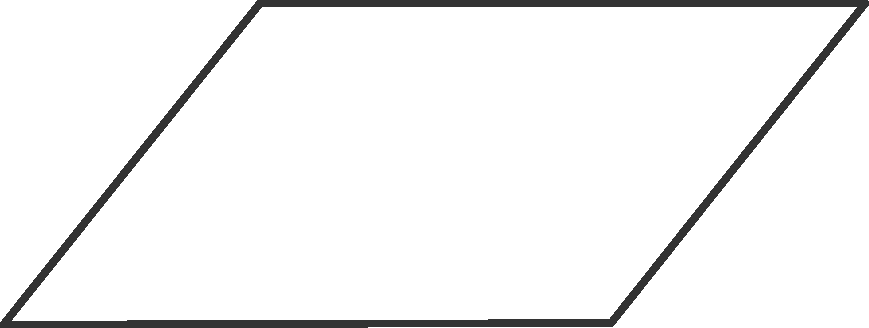
\includegraphics[width=3.5cm]{figures/curv_plan} &
      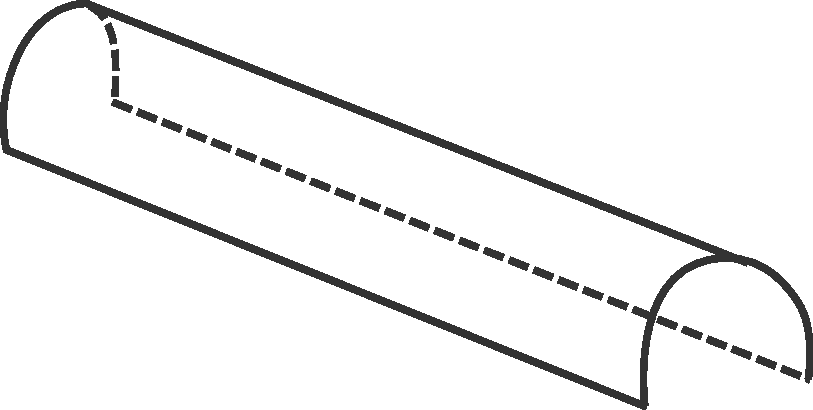
\includegraphics[width=3.5cm]{figures/curv_cylindre_conv} &
      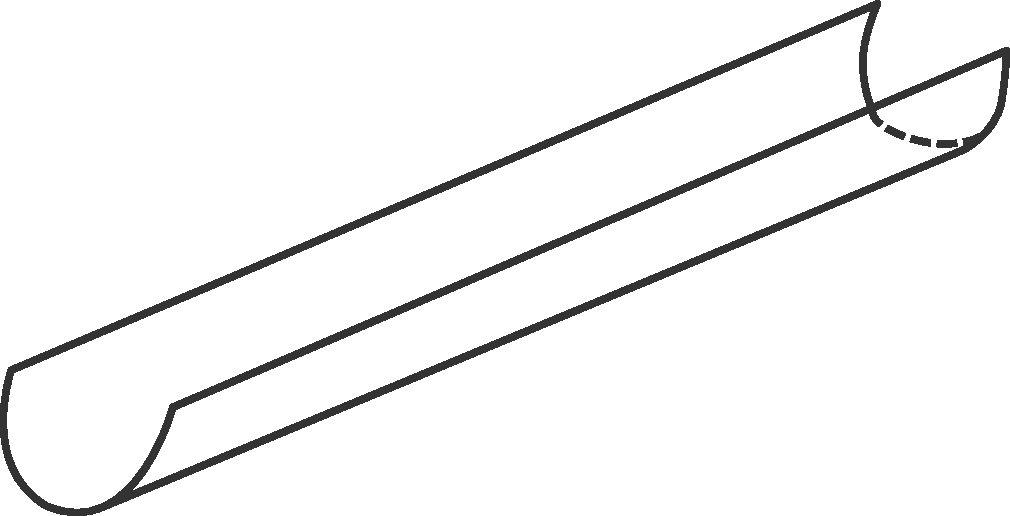
\includegraphics[width=3.5cm]{figures/curv_cylindre_conc}
      \\
      Plan &
      Cylindre convexe &
      Cylindre concave
      \\
      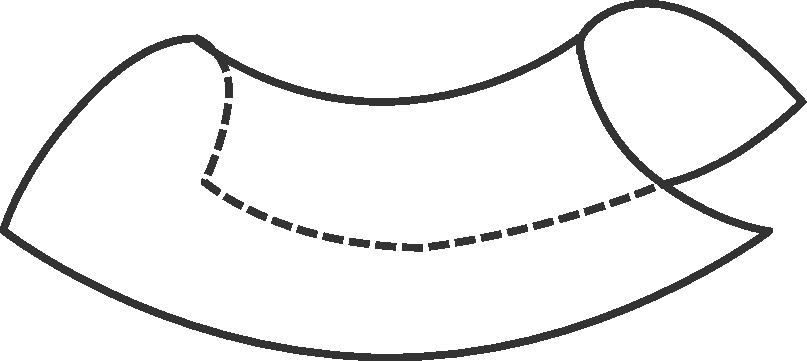
\includegraphics[width=3.5cm]{figures/curv_minimal} &
      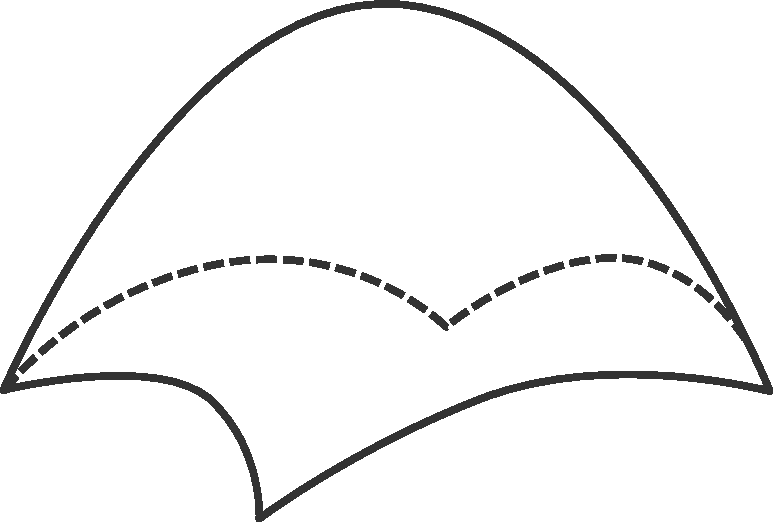
\includegraphics[width=3.5cm]{figures/curv_pic} &
      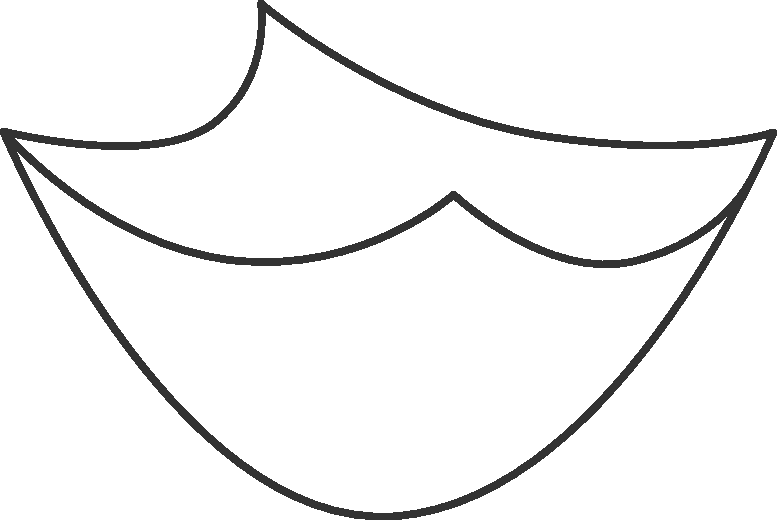
\includegraphics[width=3.5cm]{figures/curv_vallee}
      \\
      Surface minimale &
      Pic &
      Vallée
      \\
      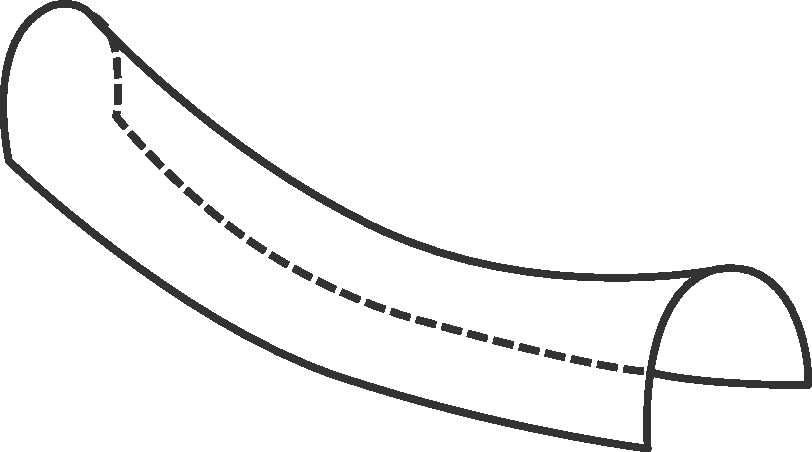
\includegraphics[width=3.5cm]{figures/curv_col_conv} &
      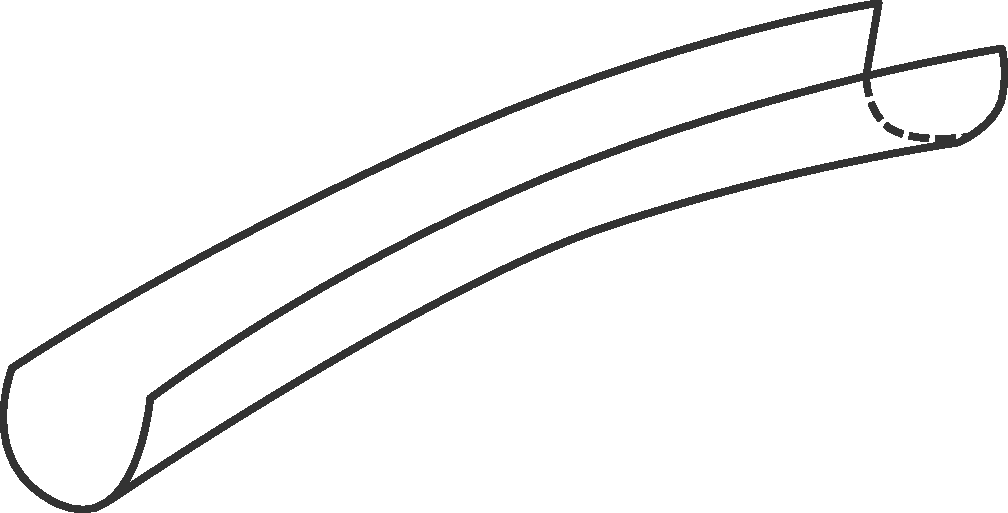
\includegraphics[width=3.5cm]{figures/curv_col_conc} &
      \\
      Col convexe &
      Col concave &
    \end{tabular}
    \caption{Illustration de différentes surfaces de dimension 3.\label{fig:curvature-figures}}
  \end{center}
\end{figure}
% \begin{figure}[ht]
%   \begin{center}
%     \input{figures/tikz/curv-osc.tikz}
%   \end{center}
%   \caption[.]
%   %
%   {.\label{fig:curvature_osc}}
%   %
% \end{figure}


En dimension 3, nous pouvons définir la courbure de la surface. Celle-ci prend
plusieurs formes : la courbure moyenne, la courbure gaussienne et les courbures
principales. Nous allons détailler cela. %%TODO

\begin{figure}[ht]{
    \begin{center}
    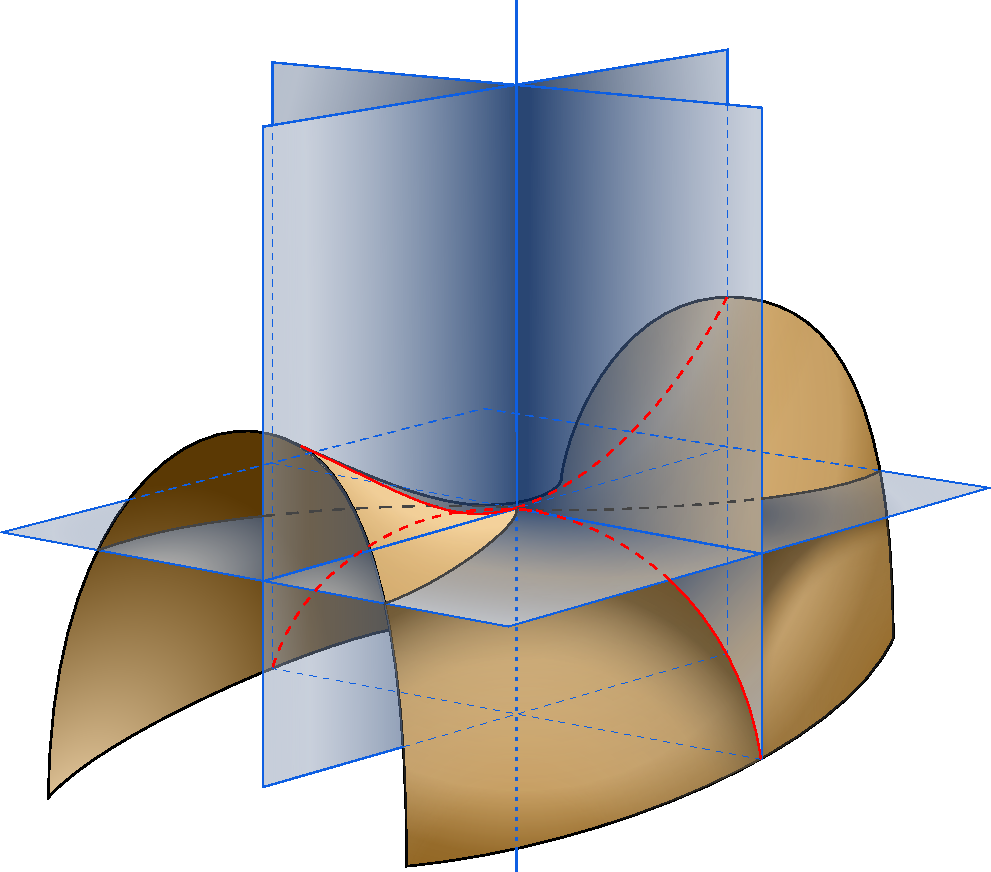
\includegraphics[width=8cm]{figures/Minimal_surface_curvature_planes-fr}
    \end{center}}
    \caption{Plans des courbures principales \cite{WikipediaCurv}.\label{fig:wiki-surv}}
\end{figure}

Considérons le \colorize{repère de Frenet} défini par la normale $\NormalDir$ et
deux vecteurs orthogonaux $\vec{t_1}$ et $\vec{t_2}$ du plan tangent au point
$\vx$ de la surface $\dS$ pour $\Shape \subset \R^3$. Dans ce repère, nous
considérons deux plans orthogonaux, $\Pi_1$ et $\Pi_2$, formant deux courbes 2D
$f_1$ et $f_2$ à l'intersection du plan et de la surface $\dS$ (voir
\RefFigure{fig:wiki-surv}). Notons $\PrincCurv{a}(\vx)$ la courbure de $f_1$ au
point $\vx$ et $\PrincCurv{b}(\vx)$ la courbure de $f_2$ au point $\vx$. Si
$f_1$ et $f_2$ sont deux fois dérivables en $\vx$, alors la \colorize{courbure
moyenne} $\MeanCurv(\vx)$ est définie comme étant :
%
\begin{equation}
  %
  \MeanCurv(\vx) = \frac{\PrincCurv{a}(\vx) + \PrincCurv{b}(\vx)}{2} \,.
  %
\end{equation}

Si $\PrincCurv{a}$ et $\PrincCurv{b}$ sont \respp la \colorize{courbure
maximale} $\PrincCurv{1}(\vx)$ et la \colorize{courbure minimale}
$\PrincCurv{2}(\vx)$ dans toutes les directions du repère de Frenet au point
$\vx$, alors nous pouvons définir la courbure gaussienne $\GaussCurv(\vx)$ comme
étant :
%
\begin{equation}
  %
  \GaussCurv(\vx) = \PrincCurv{1} \cdot \PrincCurv{2} \,.
  %
\end{equation}

% En dimension 3, nous pouvons également définir la courbure moyenne, la courbure
% gaussienne et les courbures principales. En recentrant à l'origine du repère, et
% que le plan tangent est $x_3 = 0$, nous pouvons paramétrer $f$ par une décomposition en série de Taylor \cite{Taylor1717} afin d'en extraire les
% \colorize{courbures principales} $\PrincCurv{1}$ et $\PrincCurv{2}$ :
% %
% \begin{equation}
%   %
%   f(x_1,x_2) = \frac{1}{2}\PrincCurv{1}x_1^2 + \frac{1}{2}\PrincCurv{2}x_2^2 + \cdots \,.
%   %
% \end{equation}
% %
% Alors, la \colorize{courbure moyenne} est calculée comme étant :
% %
% \begin{equation}
%   %
%   \MeanCurv(\vx) = \frac{\PrincCurv{1} + \PrincCurv{2}}{2} \,,
%   %
% \end{equation}
% %
% et la \colorize{courbure gaussienne} :
% %
% \begin{equation}
%   %
%   \GaussCurv(\vx) = \PrincCurv{1} \cdot \PrincCurv{2} \,.
%   %
% \end{equation}
%
Nous pouvons noter quelques particularités en dimension 3 :
\begin{itemize}
  \item la sphère unité a une courbure moyenne et gaussienne constante égale à $1$;
  \item le plan euclidien a une courbure moyenne et gaussienne nulle;
  \item le cylindre a une courbure moyenne positive et une courbure gaussienne nulle.
\end{itemize}
%
Le \RefTable{tab:courbure-particularities} et la
\RefFigure{fig:curvature-figures} montre une classification des surfaces de
dimension 3 en fonction du signe de leur courbure moyenne et gaussienne.


\begin{table}[ht]
\centering
\caption{Particularités des surfaces en fonction de leur courbures moyenne et gaussienne}
\label{tab:courbure-particularities}
\begin{tabular}{@{}lccc@{}}
\toprule
                  & $\GaussCurv = 0$   & $\GaussCurv > 0$   & $\GaussCurv < 0$   \\ \midrule
$\MeanCurv = 0$   & plan               & \svgNope           & surface minimale   \\
$\MeanCurv > 0$   & cylindre concave   & vallée             & col concave        \\
$\MeanCurv < 0$   & cylindre convexe   & pic                & col convexe        \\ \bottomrule
\end{tabular}
\end{table}


\section{Éléments de géométrie digitale}
\label{sec:notions-base}
%
Dans ce paragraphe, nous allons introduire les notions de bases de la géométrie
digitale comme le \colorize{pavage}. Un pavage est un ensemble de cellules
partitionnant entièrement l'espace euclidien. Il existe plusieurs types de
pavages présents dans la nature (craquement de sol sous l'effet de la chaleur,
peaux d'animaux (serpent, girafe, etc.), sol de la Chaussée des Géants
(Royaume-Uni), etc.) comme dans les constructions de l'Homme (carrelages, routes
pavées, pyramide du Louvre (Paris, France), mosaïques, vitraux, etc.), comme
l'illustre la \RefFigure{fig:pavage-exemple}.

\begin{figure}[ht]
  \begin{center}
    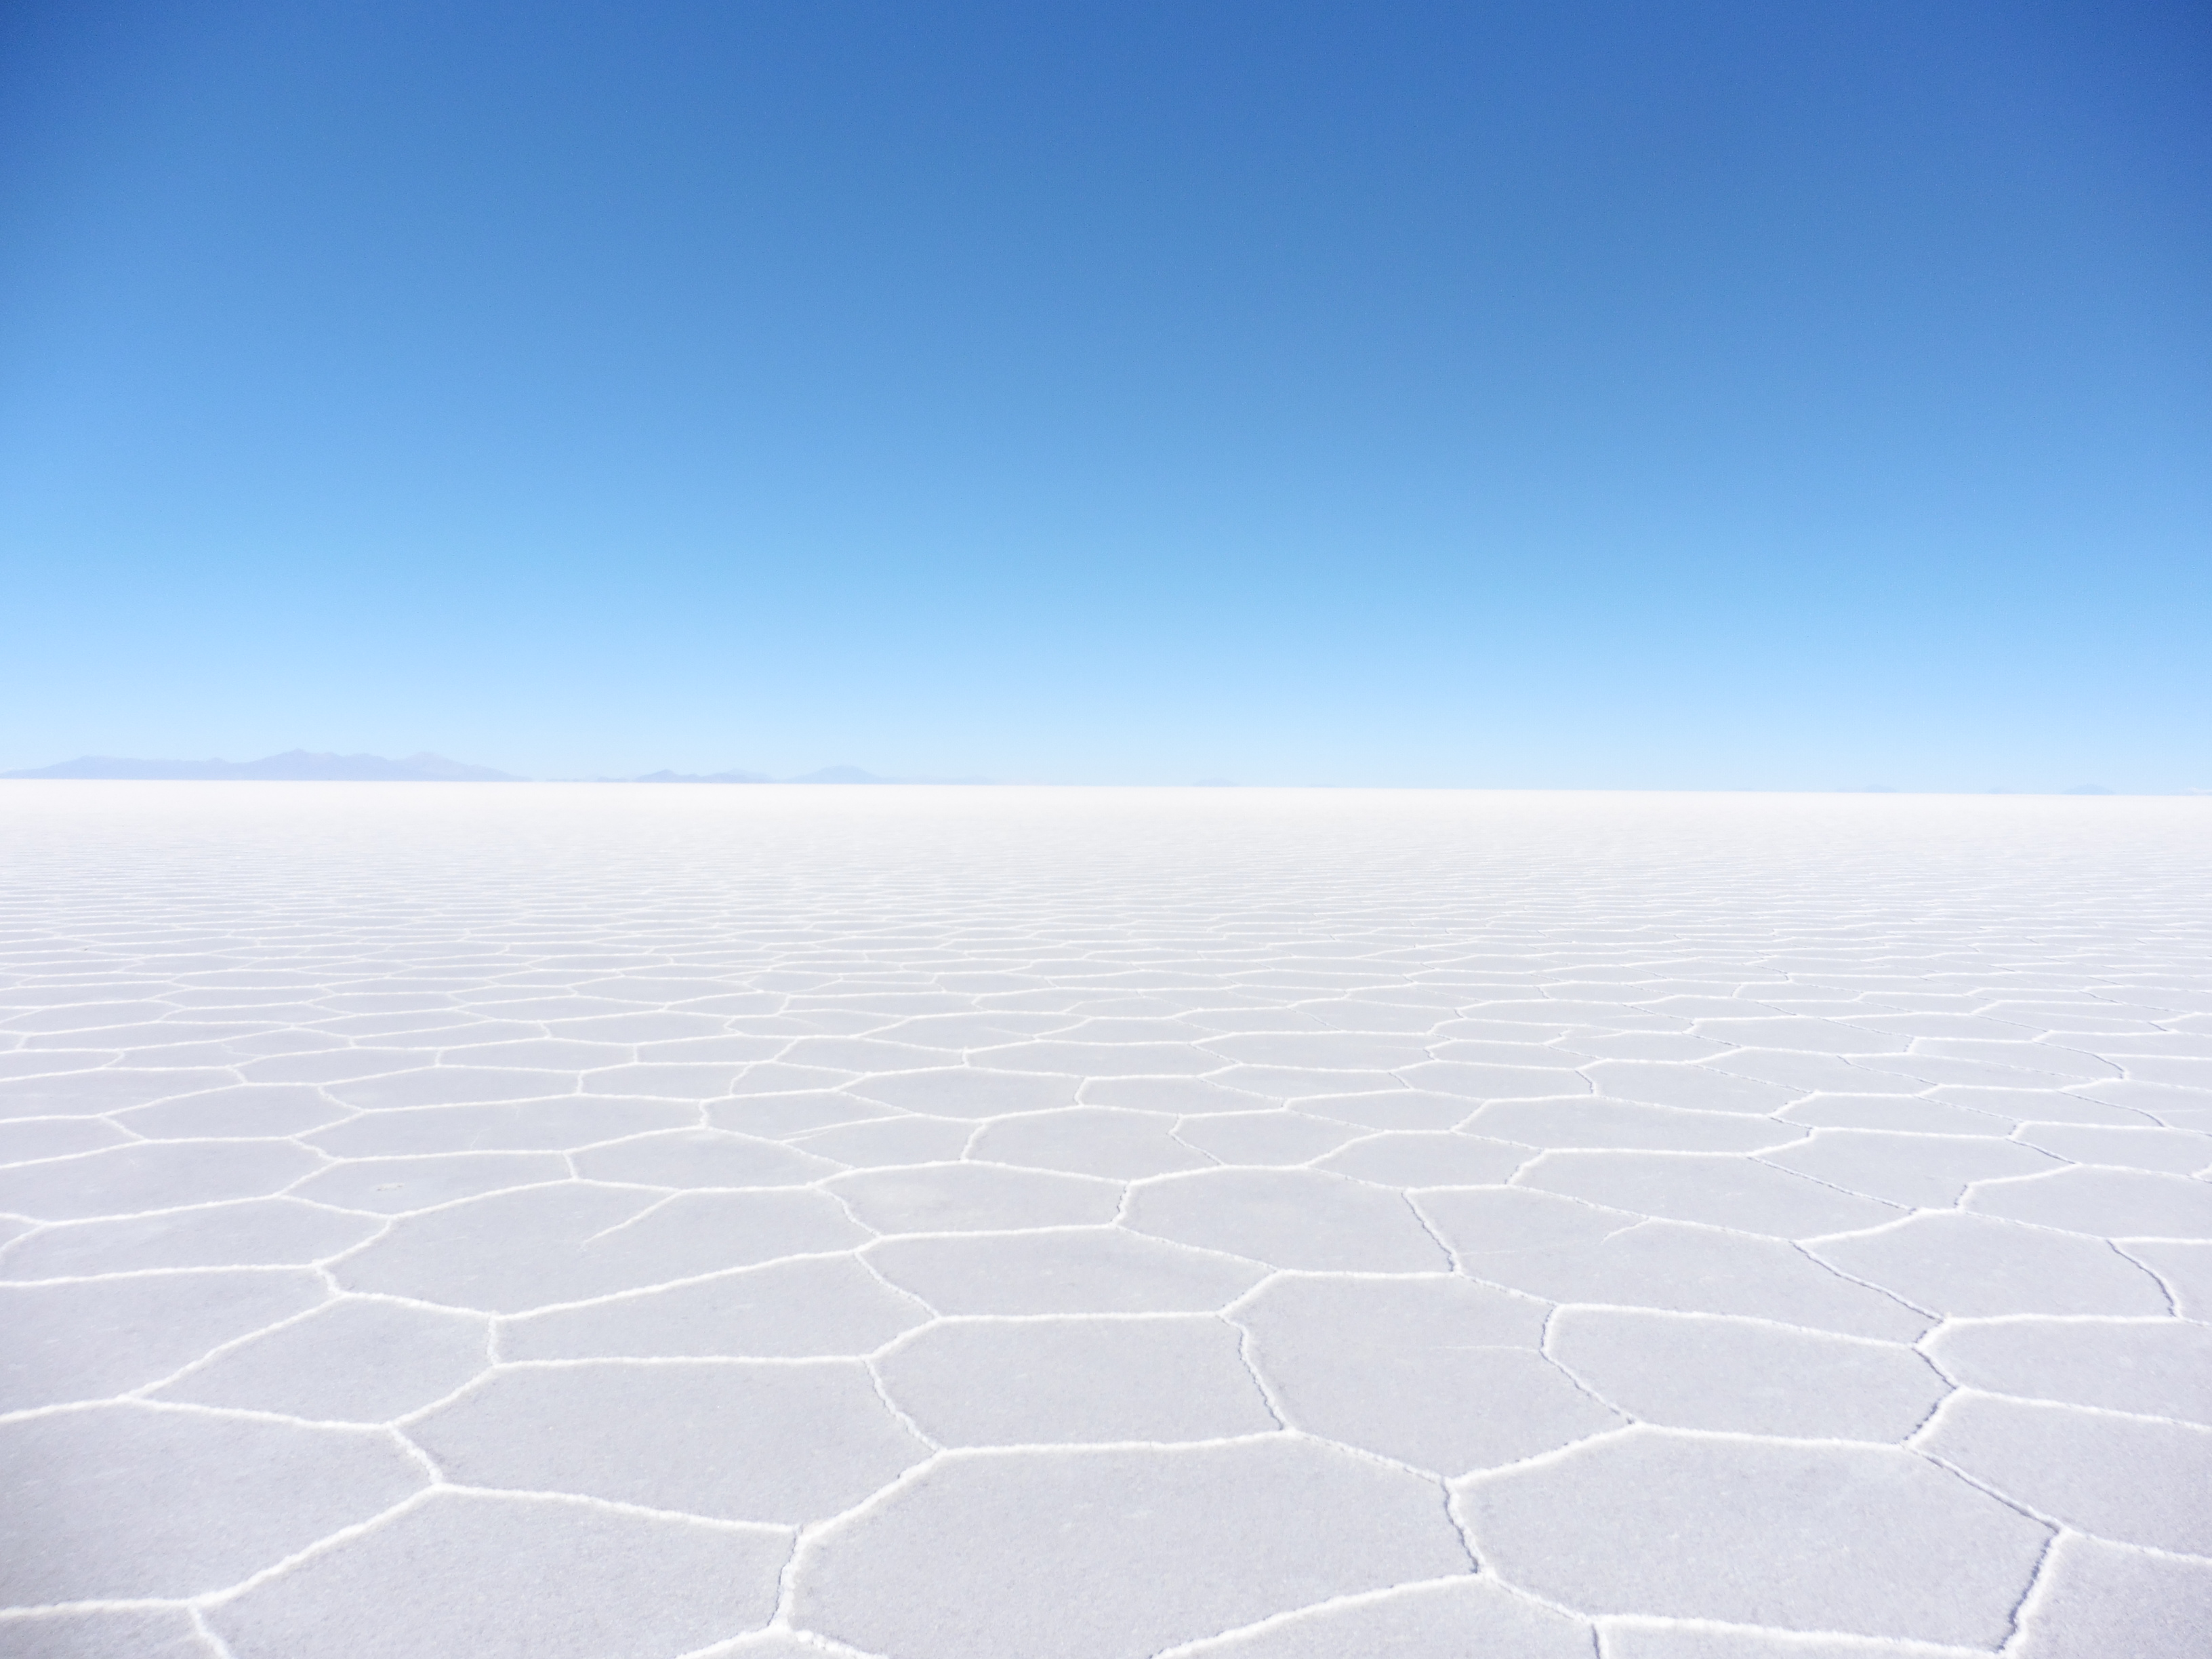
\includegraphics[width=6.8cm]{images/Notions/pavage_mer_de_sel}
    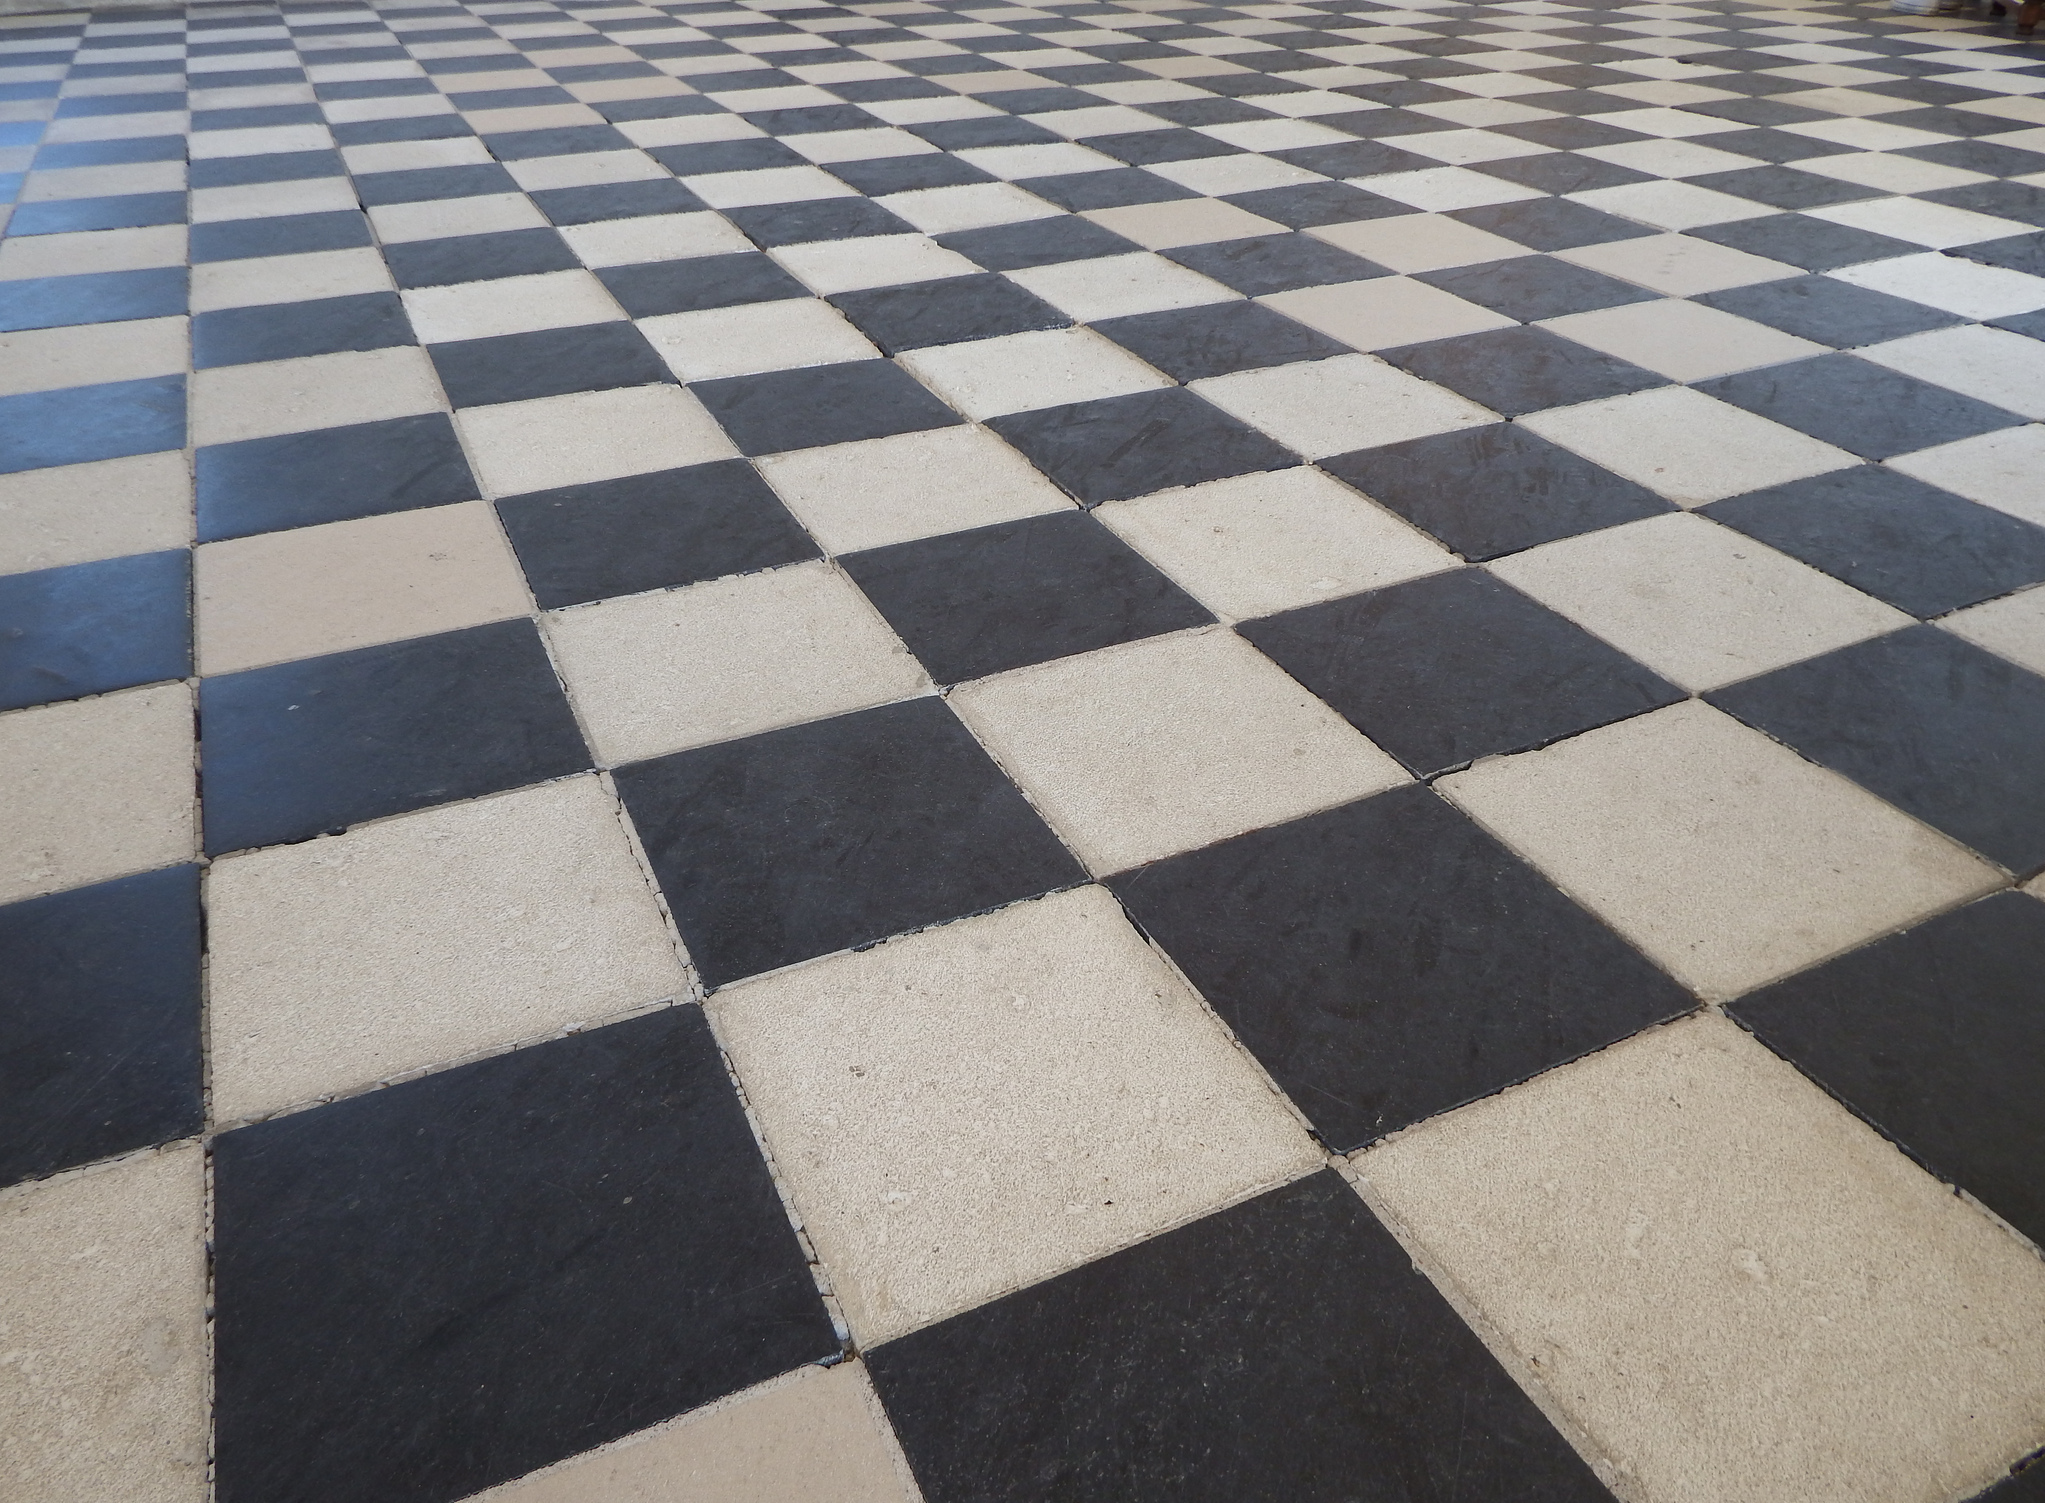
\includegraphics[width=6.8cm]{images/Notions/pavage_chateau}\\
    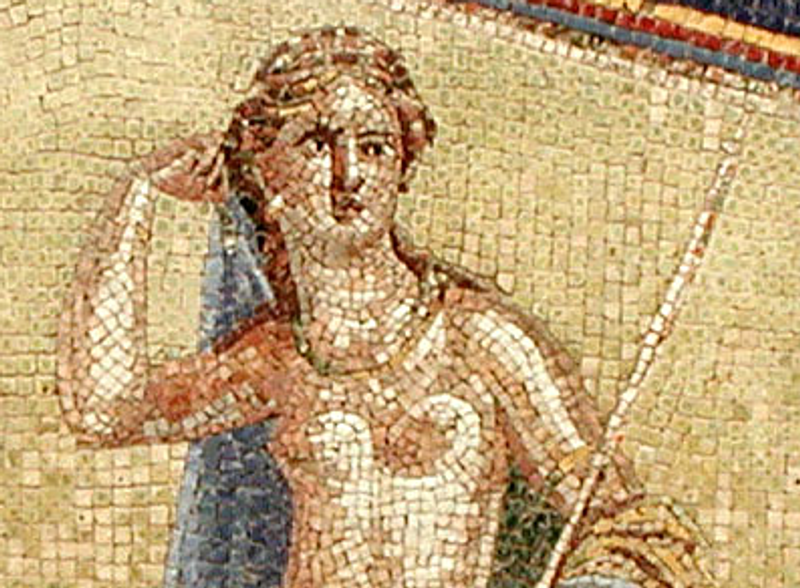
\includegraphics[width=6.8cm]{images/Notions/pavage_mosaique}
    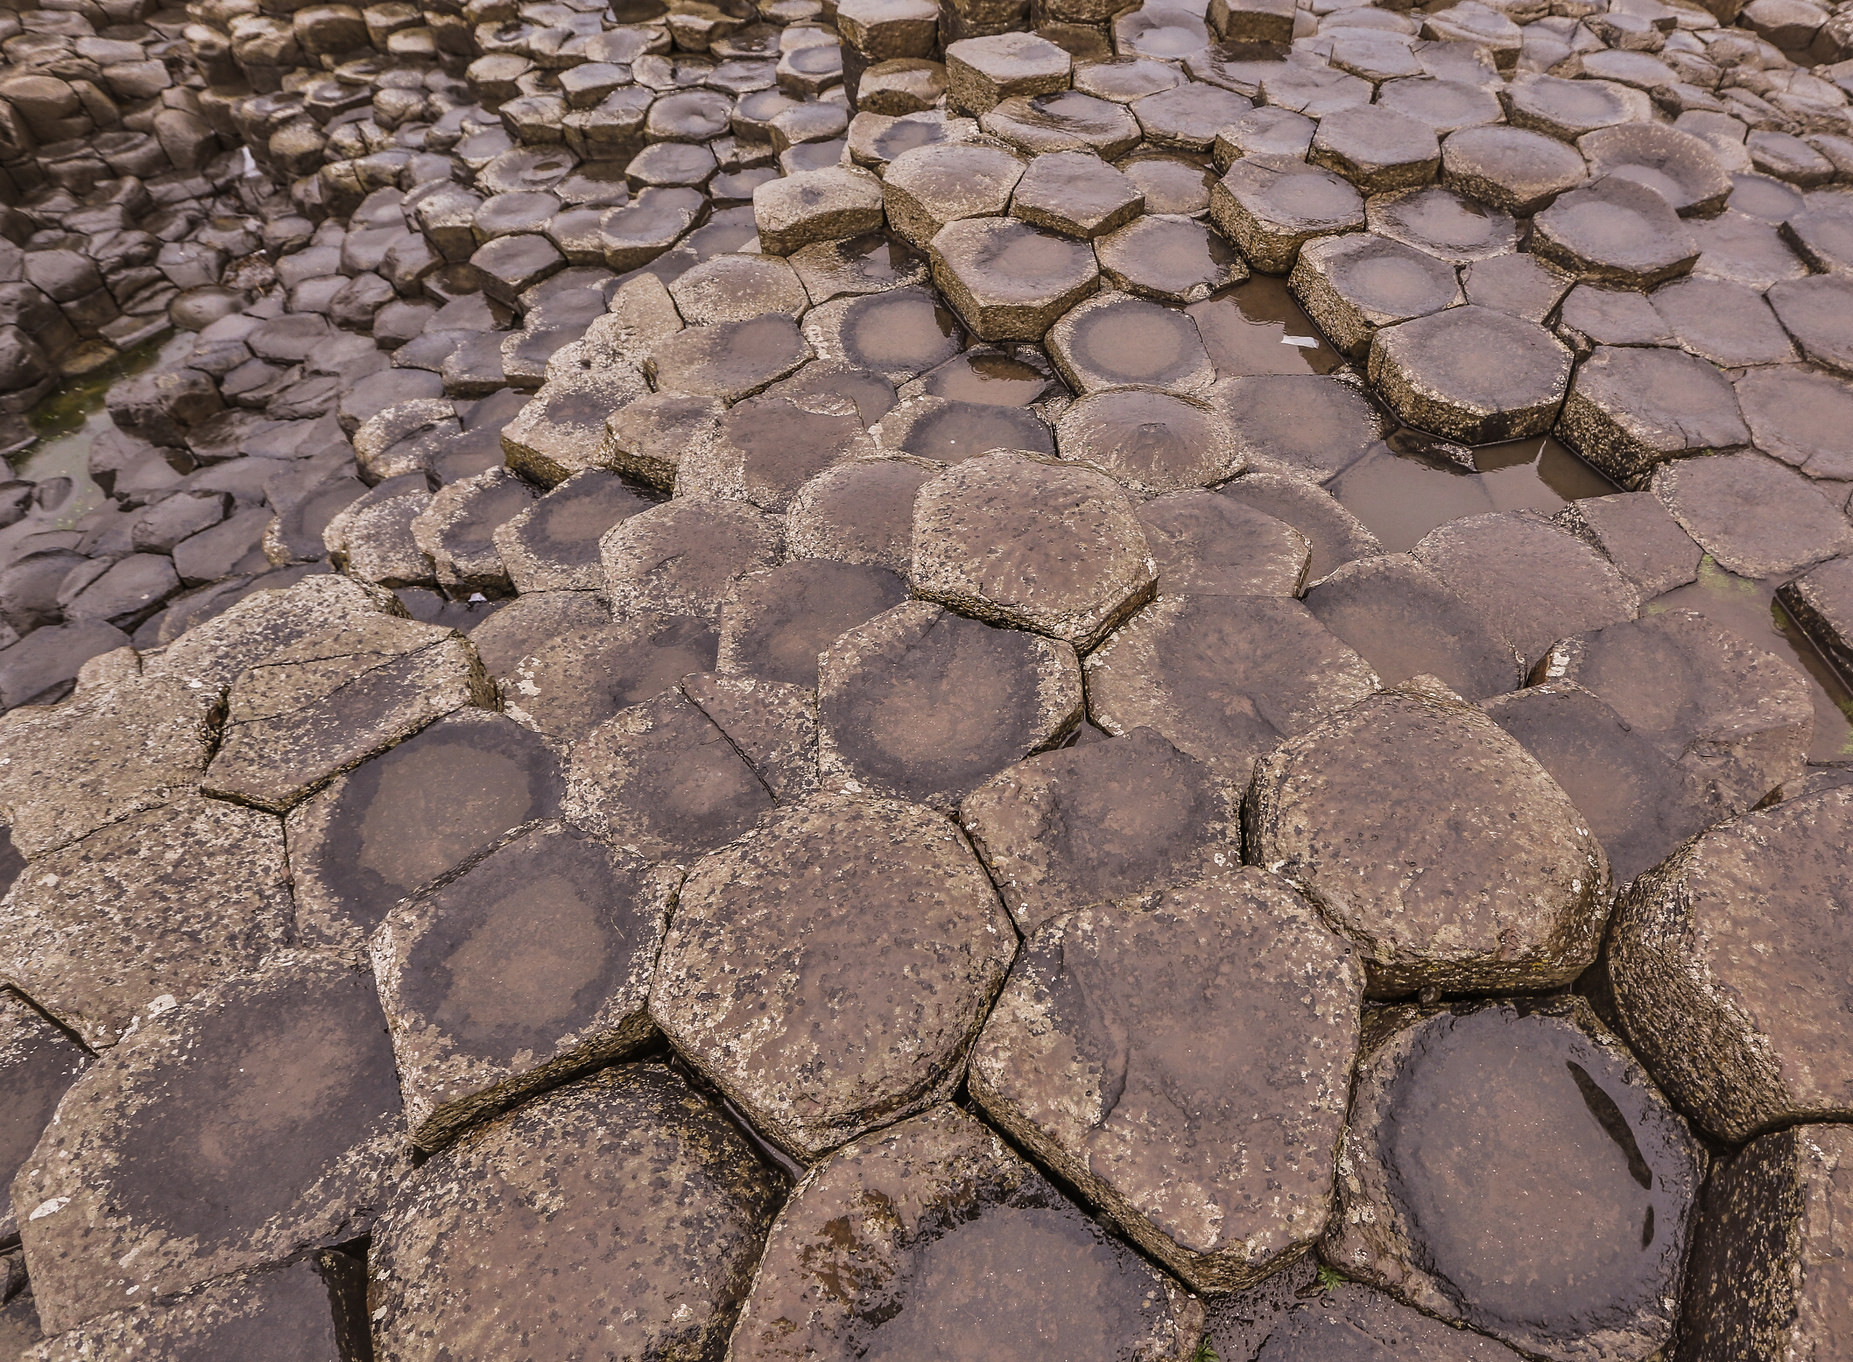
\includegraphics[width=6.8cm]{images/Notions/pavage_chaussee_des_geants}\\
    \caption[Différents pavages dans la nature ou dans les constructions humaines]
    %
    {Différents pavages dans la nature ou dans les constructions humaines.
    \emph{De gauche à droite, de haut en bas :} désert de sel en Bolivie
    \cite{pavage1}, sol d'un des châteaux de la Loire (France) \cite{pavage2},
    mosaïque représentant Amphitrite (Herculanum, Italie), formation de basalte à la Chaussée des
    Géants (Royaume-Uni) \cite{pavage4}.\label{fig:pavage-exemple}}
    %
  \end{center}
\end{figure}

Un sous-ensemble de ces pavages contient les \colorize{pavages réguliers}. Nous
appelons un \colorize{espace digital} un pavage régulier du plan en dimension 2
ou de l'espace en dimension $d > 2$. Plusieurs types de pavages réguliers
existent (voir la \RefFigure{fig:pavages}), nous nous intéressons ici uniquement
aux pavages discrets par carrés (ou des cubes en dimension supérieure). Les
points digitaux (\colorize{pixels} en dimension 2, \colorize{voxels} en
dimension 3) de ce pavage régulier isothétique (aligné sur les axes)  associés à
cet espace sont des points de $\Z^d$ comme nous pouvons le voir avec le graphe
dual de la \RefFigure{fig:pavage_dual}. Les coordonnées des points digitaux sont
alors des nombres entiers, rendant les calculs plus simples et stables qu'avec
des coordonnées réelles. Les \colorize{objets digitaux} $\DigShape \subset \Z^d$
sont alors simplement définis comme des ensembles de points digitaux de
dimension $d$.

\begin{figure}[ht]
  \begin{center}
    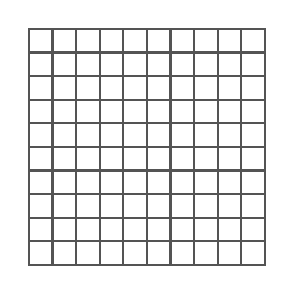
\begin{tikzpicture}[x=0.3cm,y=0.3cm]
  \definecolor{kGrey}{rgb}{0.33,0.33,0.33}

  \foreach \x/\y in { 0/0,1/0,2/0,3/0,4/0,5/0,6/0,7/0,8/0,9/0,
                      0/2,1/2,2/2,3/2,4/2,5/2,6/2,7/2,8/2,9/2,
                      0/4,1/4,2/4,3/4,4/4,5/4,6/4,7/4,8/4,9/4,
                      0/6,1/6,2/6,3/6,4/6,5/6,6/6,7/6,8/6,9/6,
                      0/8,1/8,2/8,3/8,4/8,5/8,6/8,7/8,8/8,9/8
                    }
  {
    \draw[color=kGrey,thick] (\x,\y) -- (\x+1,\y) -- (\x+1,\y+1) -- (\x,\y+1) -- cycle;
    \draw[color=kGrey,thick] (\x,\y+1) -- (\x+1,\y+1) -- (\x+1,\y+2) -- (\x,\y+2) -- cycle;
  }
\end{tikzpicture}\quad
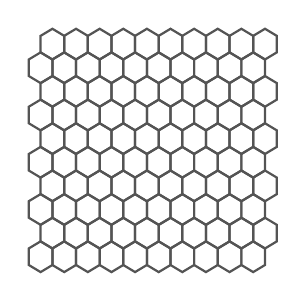
\begin{tikzpicture}[x=0.3cm,y=0.3cm]
  \definecolor{kGrey}{rgb}{0.33,0.33,0.33}

  \foreach \x/\y in { 0/0,1/0,2/0,3/0,4/0,5/0,6/0,7/0,8/0,9/0,
                      0/2,1/2,2/2,3/2,4/2,5/2,6/2,7/2,8/2,9/2,
                      0/4,1/4,2/4,3/4,4/4,5/4,6/4,7/4,8/4,9/4,
                      0/6,1/6,2/6,3/6,4/6,5/6,6/6,7/6,8/6,9/6,
                      0/8,1/8,2/8,3/8,4/8,5/8,6/8,7/8,8/8,9/8
                    }
  {
    \draw[color=kGrey,thick] (\x+0.5,\y-0.15) -- (\x+1,\y+0.15) -- (\x+1,\y+0.85) -- (\x+0.5,\y+1.15) -- (\x,\y+0.85) -- (\x,\y+0.15) -- cycle;
    \draw[color=kGrey,thick] (\x+1,\y+0.85) -- (\x+1.5,\y+1.15) -- (\x+1.5,\y+1.85) -- (\x+1,\y+2.15) -- (\x+0.5,\y+1.85) -- (\x+0.5,\y+1.15) -- cycle;
  }
\end{tikzpicture}\quad
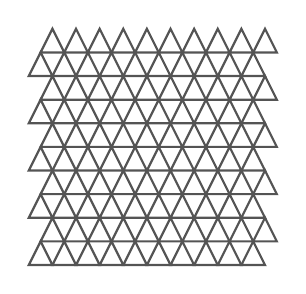
\begin{tikzpicture}[x=0.3cm,y=0.3cm]
  \definecolor{kGrey}{rgb}{0.33,0.33,0.33}

  \foreach \x/\y in { 0/0,1/0,2/0,3/0,4/0,5/0,6/0,7/0,8/0,9/0,
                      0/2,1/2,2/2,3/2,4/2,5/2,6/2,7/2,8/2,9/2,
                      0/4,1/4,2/4,3/4,4/4,5/4,6/4,7/4,8/4,9/4,
                      0/6,1/6,2/6,3/6,4/6,5/6,6/6,7/6,8/6,9/6,
                      0/8,1/8,2/8,3/8,4/8,5/8,6/8,7/8,8/8,9/8
                    }
  {
    \draw[color=kGrey,thick] (\x-0.5,\y) -- (\x+0.5,\y) -- (\x,\y+1) -- cycle;
    \draw[color=kGrey,thick] (\x,\y+1) -- (\x+1,\y+1) -- (\x+0.5,\y+2) -- cycle;
  }
\end{tikzpicture}

    \caption{Pavages 2D réguliers par carrés, hexagones et triangles (\RefFigureFake{1.1}{Coeurjolly2002}).\label{fig:pavages}}
  \end{center}
\end{figure}

\begin{figure}[ht]
  \begin{center}
    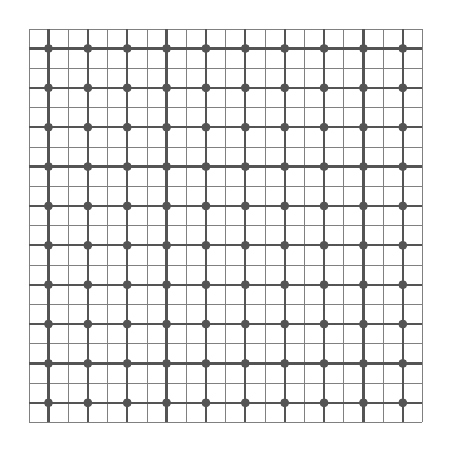
\begin{tikzpicture}[x=0.5cm,y=0.5cm]
  \definecolor{kGrey}{rgb}{0.33,0.33,0.33}

  % grids
  \draw[help lines,step=0.5cm] (0,0) grid (10,10);

  \foreach \x/\y in { 0/0,1/0,2/0,3/0,4/0,5/0,6/0,7/0,8/0,9/0,
                      0/2,1/2,2/2,3/2,4/2,5/2,6/2,7/2,8/2,9/2,
                      0/4,1/4,2/4,3/4,4/4,5/4,6/4,7/4,8/4,9/4,
                      0/6,1/6,2/6,3/6,4/6,5/6,6/6,7/6,8/6,9/6,
                      0/8,1/8,2/8,3/8,4/8,5/8,6/8,7/8,8/8,9/8
                    }
  {
    \draw[color=kGrey,thick] (\x,\y+0.5) -- (\x+1,\y+0.5);
    \draw[color=kGrey,thick] (\x,\y+1.5) -- (\x+1,\y+1.5);
    \draw[color=kGrey,thick] (\x+0.5,\y) -- (\x+0.5,\y+2); % two rows

    \draw[color=kGrey,fill] (\x+0.5,\y+0.5) circle (0.5mm);
    \draw[color=kGrey,fill] (\x+0.5,\y+1.5) circle (0.5mm);
  }
\end{tikzpicture}\quad

    \caption{Dual du pavage 2D réguliers par carrés.\label{fig:pavage_dual}}
  \end{center}
\end{figure}

De ces points digitaux, nous pouvons ajouter des informations topologiques en
considérant l'espace de grille cellulaire ou inter-pixels. L'idée est de plonger
l'espace digital $\Z^n$ dans l'espace cubique cartésien afin de pouvoir
représenter les éléments inter-pixels \cite{Kovalesvsky1989, Khalimsky1990,
Francon1991}, que nous nommerons \colorize{topologie de Khalimsky}. Ainsi :
%
\begin{itemize}
%
  \item Les $0$-cellules sont appelées des \colorize{pointels} (éléments
  de dimension 0);
%
  \item Les $1$-cellules sont appelées des \colorize{lignels} ou
  \anglais{linels} (éléments de dimension 1);
%
  \item Les $2$-cellules sont appelées des \colorize{pixels} (éléments de
  dimension 2).
%
  \item Les $3$-cellules sont appelées des \colorize{voxels} (éléments de
  dimension 3).
%
\end{itemize}

\begin{figure}[ht]
  \begin{center}
    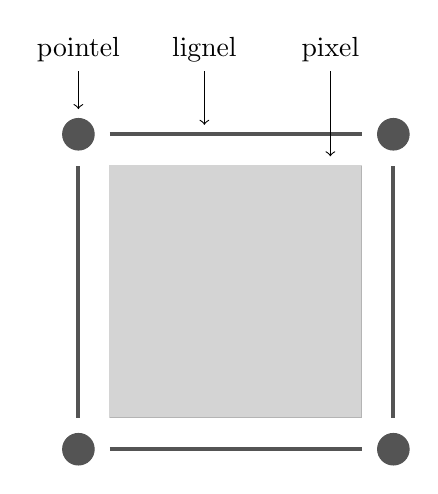
\begin{tikzpicture}[x=0.4cm,y=0.4cm]
  \definecolor{kGrey}{rgb}{0.33,0.33,0.33}

  \draw[color=kGrey,fill, nearly transparent] (1,1) rectangle (9,9);

  \draw[color=kGrey,fill] (0,0) circle (0.5);
  \draw[color=kGrey,fill] (10,0) circle (0.5);
  \draw[color=kGrey,fill] (0,10) circle (0.5);
  \draw[color=kGrey,fill] (10,10) circle (0.5);

  \draw[color=kGrey,thick,line width=0.5mm] (1,0) -- (9,0);
  \draw[color=kGrey,thick,line width=0.5mm] (1,10) -- (9,10);
  \draw[color=kGrey,thick,line width=0.5mm] (0,1) -- (0,9);
  \draw[color=kGrey,thick,line width=0.5mm] (10,1) -- (10,9);

  \draw[<-,black] (0,10.8) -- (0,12)  node[above] {pointel};
  \draw[<-,black] (4,10.3) -- (4,12)  node[above] {lignel};
  \draw[<-,black] (8,9.3) -- (8,12)  node[above] {pixel};

\end{tikzpicture}
%\begin{tikzpicture}[x=0.4cm,y=0.4cm]
%  \definecolor{kGrey}{rgb}{0.33,0.33,0.33}
%
%  \draw[color=kGrey,fill, nearly transparent] (1,1) rectangle (9,9);
%
%  \draw[color=kGrey,thick,fill=kGrey, nearly transparent] (10.7,1.7) -- (14.3,5.3) -- (14.3,13.3) -- (10.7,9.7) -- cycle;
%
%  \draw[color=kGrey,fill] (0,0) circle (0.5);
%  \draw[color=kGrey,fill] (10,0) circle (0.5);
%  \draw[color=kGrey,fill] (0,10) circle (0.5);
%  \draw[color=kGrey,fill] (10,10) circle (0.5);
%
%  \draw[color=kGrey,fill] (15,5) circle (0.5);
%  \draw[color=kGrey,fill] (15,15) circle (0.5);
%  \draw[color=kGrey,fill] (5,15) circle (0.5);
%
%  \draw[color=kGrey,thick,line width=0.5mm] (1,0) -- (9,0);
%  \draw[color=kGrey,thick,line width=0.5mm] (1,10) -- (9,10);
%  \draw[color=kGrey,thick,line width=0.5mm] (0,1) -- (0,9);
%  \draw[color=kGrey,thick,line width=0.5mm] (10,1) -- (10,9);
%
%  \draw[color=kGrey,thick,line width=0.5mm] (11,1) -- (14,4);
%  \draw[color=kGrey,thick,line width=0.5mm] (11,11) -- (14,14);
%  \draw[color=kGrey,thick,line width=0.5mm] (15,6) -- (15,14);
%  \draw[color=kGrey,thick,line width=0.5mm] (1,11) -- (4,14);
%  \draw[color=kGrey,thick,line width=0.5mm] (6,15) -- (14,15);
%
%  \draw[<-,black] (0,10.8) -- (0,12)  node[above] {pointel};
%  \draw[<-,black] (4,10.3) -- (4,12)  node[above] {lignel};
%  \draw[<-,black] (8,9.3) -- (8,12)  node[above] {pixel};
%
%\end{tikzpicture}

    \caption{Illustration des $0$-cellules (pointels), $1$-cellules (lignels) et
    $2$-cellules (pixels).\label{fig:notations_topo}}
  \end{center}
\end{figure}

La \RefFigure{fig:notations_topo} illustre les pointels, lignels et pixels. Par
convention, nous nommons les $n$-cellules les \colorize{spels} (un pixel en
dimension 2, un voxel en dimension 3), les $n-1$-cellules sont nommées les
\colorize{bels} ou \colorize{surfel} pour \anglais{surface elements} (un
\colorize{lignel} en dimension 2, un \colorize{pixel} en dimension 3). Par
convention, les points digitaux $\vp \in \Z^d$ sont plongés dans des
spels.


%
% \subsection{Voisinages}
% \label{sec:voisinage}
%
Grâce à ces définitions, cela nous amène directement aux questions de voisinage
des points digitaux. La relation de voisinage est une notion importante pour la
définition de notre objet digital. Le voisinage est défini en fonction de la
\colorize{connexité} que possède une cellule digitale par rapport aux autres.
Les \RefTablesN{tab:adjacence2d}{tab:adjacence3d} définissent formellement ces
notions, et la \RefFigure{fig:adjacence2d} illustre la $4$-connexité et la
$8$-connexité sur un objet digital de dimension 2. Un autre terme désigne cette
notion de voisinage : \colorize{l'adjacence}. Ainsi, nous parlons de
$n$-adjacence pour les liens entre éléments de dimension $n$ (\cad les pointels
pour $n=0$, les lignels pour $n=1$ en dimension 2).

\begin{table}[ht]
  \centering
  \caption{Définition des voisinages en dimension $2$.}
  \label{tab:adjacence2d}
    \renewcommand{\arraystretch}{1.1}
  \begin{tabular}{@{}llr@{}}
    \toprule
    Adjacence & Connexité  & Caractérisation \\ \midrule
    $1$ & $4$        & $||\vx - \vy||_1 = 1$ \\
    $0$ & $8$        & $||\vx - \vy||_\infty = 1$ \\
    \bottomrule
  \end{tabular}
\end{table}

\begin{table}[ht]
  \centering
  \caption{Définition des voisinages en dimension $3$.}
  \label{tab:adjacence3d}
    \renewcommand{\arraystretch}{1.1}
  \begin{tabular}{@{}llr@{}}
    \toprule
    Adjacence & Connexité  & Caractérisation \\ \midrule
    $2$ & $6$        & $||\vx - \vy||_1 = 1$ \\
    $1$ & $18$       & $||\vx - \vy||_\infty = 1$ et $||\vx - \vy||_1 \le 2$ \\
    $0$ & $26$       & $||\vx - \vy||_\infty = 1$ \\
    \bottomrule
  \end{tabular}
\end{table}

\begin{figure}[ht]
  \begin{center}
    %
% Sometimes, Tikz is not the best choice ....
%
%
%
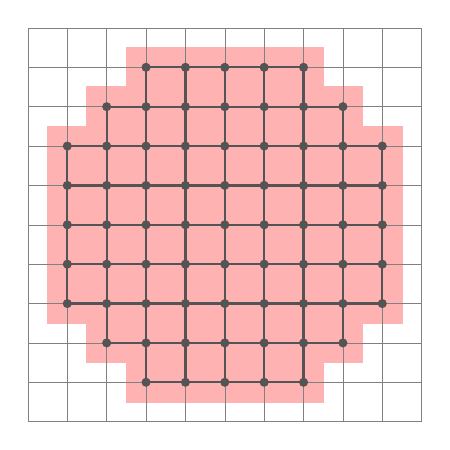
\begin{tikzpicture}[x=0.5cm,y=0.5cm]
  \definecolor{kGrey}{rgb}{0.33,0.33,0.33}

  % Cells
  \foreach \x/\y in {
                                  3/1,4/1,5/1,6/1,7/1,
                              2/2,3/2,4/2,5/2,6/2,7/2,8/2,
                          1/3,2/3,3/3,4/3,5/3,6/3,7/3,8/3,9/3,
                          1/4,2/4,3/4,4/4,5/4,6/4,7/4,8/4,9/4,
                          1/5,2/5,3/5,4/5,5/5,6/5,7/5,8/5,9/5,
                          1/6,2/6,3/6,4/6,5/6,6/6,7/6,8/6,9/6,
                          1/7,2/7,3/7,4/7,5/7,6/7,7/7,8/7,9/7,
                              2/8,3/8,4/8,5/8,6/8,7/8,8/8,
                                  3/9,4/9,5/9,6/9,7/9
                    }
  {
    \draw[color=red!30!white,fill] (\x-0.5,\y-0.5) rectangle (\x+0.5,\y+0.5);
  }

  % grids
  \draw[help lines,step=0.5cm] (0,0) grid (10,10);

  % points - connexity
  \foreach \x/\y in {
                                  3/2,4/2,5/2,6/2,7/2,
                              2/3,3/3,4/3,5/3,6/3,7/3,8/3,
                              2/4,3/4,4/4,5/4,6/4,7/4,8/4,
                              2/5,3/5,4/5,5/5,6/5,7/5,8/5,
                              2/6,3/6,4/6,5/6,6/6,7/6,8/6,
                              2/7,3/7,4/7,5/7,6/7,7/7,8/7,
                                  3/8,4/8,5/8,6/8,7/8
                    }
  {

    \draw[color=kGrey,fill] (\x,\y) circle (0.5mm);
    \draw[color=kGrey,thick] (\x-1,\y) -- (\x+1,\y);
    \draw[color=kGrey,thick] (\x,\y-1) -- (\x,\y+1);
  }

  % border points - connexity
  %% horizontal
  \foreach \x/\y in {
                                      4/1,5/1,6/1,
                                      4/9,5/9,6/9
                    }
  {

    \draw[color=kGrey,fill] (\x,\y) circle (0.5mm);
    \draw[color=kGrey,thick] (\x-1,\y) -- (\x+1,\y);
  }

  %% vertical
  \foreach \x/\y in {
                              1/4,9/4,
                              1/5,9/5,
                              1/6,9/6
                    }
  {

    \draw[color=kGrey,fill] (\x,\y) circle (0.5mm);
    \draw[color=kGrey,thick] (\x,\y-1) -- (\x,\y+1);
  }

  %% Special points
  \draw[color=kGrey,fill] (7,1) circle (0.5mm);
  \draw[color=kGrey,fill] (8,2) circle (0.5mm);
  \draw[color=kGrey,fill] (9,3) circle (0.5mm);
  %\draw[color=kGrey,thick] (7,1) -- (9,3);

  \draw[color=kGrey,fill] (7,9) circle (0.5mm);
  \draw[color=kGrey,fill] (8,8) circle (0.5mm);
  \draw[color=kGrey,fill] (9,7) circle (0.5mm);
  %\draw[color=kGrey,thick] (7,9) -- (9,7);

  \draw[color=kGrey,fill] (1,3) circle (0.5mm);
  \draw[color=kGrey,fill] (2,2) circle (0.5mm);
  \draw[color=kGrey,fill] (3,1) circle (0.5mm);
  %\draw[color=kGrey,thick] (1,3) -- (3,1);

  \draw[color=kGrey,fill] (1,7) circle (0.5mm);
  \draw[color=kGrey,fill] (2,8) circle (0.5mm);
  \draw[color=kGrey,fill] (3,9) circle (0.5mm);
  %\draw[color=kGrey,thick] (1,7) -- (3,9);
\end{tikzpicture}\quad
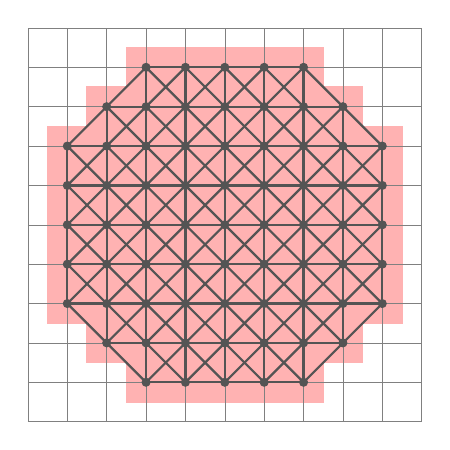
\begin{tikzpicture}[x=0.5cm,y=0.5cm]
  \definecolor{kGrey}{rgb}{0.33,0.33,0.33}

  % Cells
  \foreach \x/\y in {
                                  3/1,4/1,5/1,6/1,7/1,
                              2/2,3/2,4/2,5/2,6/2,7/2,8/2,
                          1/3,2/3,3/3,4/3,5/3,6/3,7/3,8/3,9/3,
                          1/4,2/4,3/4,4/4,5/4,6/4,7/4,8/4,9/4,
                          1/5,2/5,3/5,4/5,5/5,6/5,7/5,8/5,9/5,
                          1/6,2/6,3/6,4/6,5/6,6/6,7/6,8/6,9/6,
                          1/7,2/7,3/7,4/7,5/7,6/7,7/7,8/7,9/7,
                              2/8,3/8,4/8,5/8,6/8,7/8,8/8,
                                  3/9,4/9,5/9,6/9,7/9
                    }
  {
    \draw[color=red!30!white,fill] (\x-0.5,\y-0.5) rectangle (\x+0.5,\y+0.5);
  }

  % grids
  \draw[help lines,step=0.5cm] (0,0) grid (10,10);

  % points - connexity
  \foreach \x/\y in {
                                      4/2,5/2,6/2,
                                  3/3,4/3,5/3,6/3,7/3,
                              2/4,3/4,4/4,5/4,6/4,7/4,8/4,
                              2/5,3/5,4/5,5/5,6/5,7/5,8/5,
                              2/6,3/6,4/6,5/6,6/6,7/6,8/6,
                                  3/7,4/7,5/7,6/7,7/7,
                                      4/8,5/8,6/8
                    }
  {

    \draw[color=kGrey,fill] (\x,\y) circle (0.5mm);
    \draw[color=kGrey,thick] (\x-1,\y) -- (\x+1,\y);
    \draw[color=kGrey,thick] (\x,\y-1) -- (\x,\y+1);
    \draw[color=kGrey,thick] (\x-0.5,\y-0.5) -- (\x+0.5,\y+0.5);
    \draw[color=kGrey,thick] (\x-0.5,\y+0.5) -- (\x+0.5,\y-0.5);
  }

  % border points - connexity
  %% horizontal
  \foreach \x/\y in { 4/1,5/1,6/1 }
  {
    \draw[color=kGrey,fill] (\x,\y) circle (0.5mm);
    \draw[color=kGrey,thick] (\x-1,\y) -- (\x+1,\y);
    \draw[color=kGrey,thick] (\x,\y) -- (\x-0.5,\y+0.5);
    \draw[color=kGrey,thick] (\x,\y) -- (\x+0.5,\y+0.5);
  }
  \foreach \x/\y in { 4/9,5/9,6/9 }
  {

    \draw[color=kGrey,fill] (\x,\y) circle (0.5mm);
    \draw[color=kGrey,thick] (\x-1,\y) -- (\x+1,\y);
    \draw[color=kGrey,thick] (\x,\y) -- (\x-0.5,\y-0.5);
    \draw[color=kGrey,thick] (\x,\y) -- (\x+0.5,\y-0.5);
  }

  %% vertical
  \foreach \x/\y in { 1/4,1/5,1/6 }
  {
    \draw[color=kGrey,fill] (\x,\y) circle (0.5mm);
    \draw[color=kGrey,thick] (\x,\y-1) -- (\x,\y+1);
    \draw[color=kGrey,thick] (\x,\y) -- (\x+0.5,\y-0.5);
    \draw[color=kGrey,thick] (\x,\y) -- (\x+0.5,\y+0.5);
  }
  \foreach \x/\y in { 9/4,9/5,9/6 }
  {

    \draw[color=kGrey,fill] (\x,\y) circle (0.5mm);
    \draw[color=kGrey,thick] (\x,\y-1) -- (\x,\y+1);
    \draw[color=kGrey,thick] (\x,\y) -- (\x-0.5,\y-0.5);
    \draw[color=kGrey,thick] (\x,\y) -- (\x-0.5,\y+0.5);
  }

  %% Special points
  \draw[color=kGrey,fill] (7,1) circle (0.5mm);
  \draw[color=kGrey,fill] (8,2) circle (0.5mm);
  \draw[color=kGrey,fill] (9,3) circle (0.5mm);
  \draw[color=kGrey,thick] (7,1) -- (9,3);
  \draw[color=kGrey,thick] (7,1) -- (6.5,1.5);
  \draw[color=kGrey,thick] (8,2) -- (7.5,2.5);
  \draw[color=kGrey,thick] (9,3) -- (8.5,3.5);

  \draw[color=kGrey,fill] (7,9) circle (0.5mm);
  \draw[color=kGrey,fill] (8,8) circle (0.5mm);
  \draw[color=kGrey,fill] (9,7) circle (0.5mm);
  \draw[color=kGrey,thick] (7,9) -- (9,7);
  \draw[color=kGrey,thick] (7,9) -- (6.5,8.5);
  \draw[color=kGrey,thick] (8,8) -- (7.5,7.5);
  \draw[color=kGrey,thick] (9,7) -- (8.5,6.5);

  \draw[color=kGrey,fill] (1,3) circle (0.5mm);
  \draw[color=kGrey,fill] (2,2) circle (0.5mm);
  \draw[color=kGrey,fill] (3,1) circle (0.5mm);
  \draw[color=kGrey,thick] (1,3) -- (3,1);
  \draw[color=kGrey,thick] (1,3) -- (1.5,3.5);
  \draw[color=kGrey,thick] (2,2) -- (2.5,2.5);
  \draw[color=kGrey,thick] (3,1) -- (3.5,1.5);

  \draw[color=kGrey,fill] (1,7) circle (0.5mm);
  \draw[color=kGrey,fill] (2,8) circle (0.5mm);
  \draw[color=kGrey,fill] (3,9) circle (0.5mm);
  \draw[color=kGrey,thick] (1,7) -- (3,9);
  \draw[color=kGrey,thick] (1,7) -- (1.5,6.5);
  \draw[color=kGrey,thick] (2,8) -- (2.5,7.5);
  \draw[color=kGrey,thick] (3,9) -- (3.5,8.5);

  \draw[color=kGrey,fill] (2,3) circle (0.5mm);
  \draw[color=kGrey,fill] (3,2) circle (0.5mm);
  \draw[color=kGrey,thick] (1.5,3.5) -- (3.5,1.5);
  \draw[color=kGrey,thick] (2,3) -- (2.5,3.5);
  \draw[color=kGrey,thick] (3,2) -- (3.5,2.5);
  \draw[color=kGrey,thick] (3,2) -- (2,2);
  \draw[color=kGrey,thick] (3,2) -- (3,1);
  \draw[color=kGrey,thick] (2,3) -- (1,3);
  \draw[color=kGrey,thick] (2,3) -- (2,2);

  \draw[color=kGrey,fill] (2,7) circle (0.5mm);
  \draw[color=kGrey,fill] (3,8) circle (0.5mm);
  \draw[color=kGrey,thick] (2,7) -- (2.5,6.5);
  \draw[color=kGrey,thick] (2,7) -- (2,8);
  \draw[color=kGrey,thick] (2,7) -- (1,7);
  \draw[color=kGrey,thick] (3.5,8.5) -- (1.5,6.5);
  \draw[color=kGrey,thick] (3,8) -- (2,8);
  \draw[color=kGrey,thick] (3,8) -- (3,9);
  \draw[color=kGrey,thick] (3,8) -- (3.5,7.5);

  \draw[color=kGrey,fill] (7,2) circle (0.5mm);
  \draw[color=kGrey,fill] (8,3) circle (0.5mm);
  \draw[color=kGrey,thick] (7,2) -- (6.5,2.5);
  \draw[color=kGrey,thick] (7,2) -- (8,2);
  \draw[color=kGrey,thick] (7,2) -- (7,1);
  \draw[color=kGrey,thick] (8.5,3.5) -- (6.5,1.5);
  \draw[color=kGrey,thick] (8,3) -- (8,2);
  \draw[color=kGrey,thick] (8,3) -- (9,3);
  \draw[color=kGrey,thick] (8,3) -- (7.5,3.5);

  \draw[color=kGrey,fill] (7,8) circle (0.5mm);
  \draw[color=kGrey,fill] (8,7) circle (0.5mm);
  \draw[color=kGrey,thick] (7,8) -- (6.5,7.5);
  \draw[color=kGrey,thick] (7,8) -- (7,9);
  \draw[color=kGrey,thick] (7,8) -- (8,8);
  \draw[color=kGrey,thick] (8.5,6.5) -- (6.5,8.5);
  \draw[color=kGrey,thick] (8,7) -- (8,8);
  \draw[color=kGrey,thick] (8,7) -- (9,7);
  \draw[color=kGrey,thick] (8,7) -- (7.5,6.5);


\end{tikzpicture}

    \caption{Illustation du voisinage en dimension 2. \emph{À gauche :}
    $4$-connexité, \emph{à droite :} $8$-connexité.\label{fig:adjacence2d}}
  \end{center}
\end{figure}


Pour résumer, en dimension 2 :
%
\begin{itemize}
  %
  \item la $4$-connexité (ou $1$-adjacence) est la relation de voisinage par les
  arêtes (à gauche sur la \RefFigure{fig:adjacence2d});
  %
  \item la $8$-connexité (ou $0$-adjacence) est la relation de voisinage par les
  arêtes et les sommets (à droite sur la \RefFigure{fig:adjacence2d}).
  %
\end{itemize}
%
De même, en dimension 3 :
%
\begin{itemize}
  %
  \item la $6$-connexité (ou $2$-adjacence) est la relation de voisinage par les
  faces;
  %
  \item la $18$-connexité (ou $1$-adjacence) est la relation de voisinage par
  les faces et les arêtes.
  %
  \item la $26$-connexité (ou $0$-adjacence) est la relation de voisinage par
  les faces, les arêtes et les sommets.
  %
\end{itemize}


La notion de voisinage est alors importante. En effet, en fonction de la
connexité de l'espace digital, différentes composantes connexes peuvent être
extraites comme le montre la \RefFigure{fig:connexite}.

\begin{figure}[ht]
  \begin{center}
    
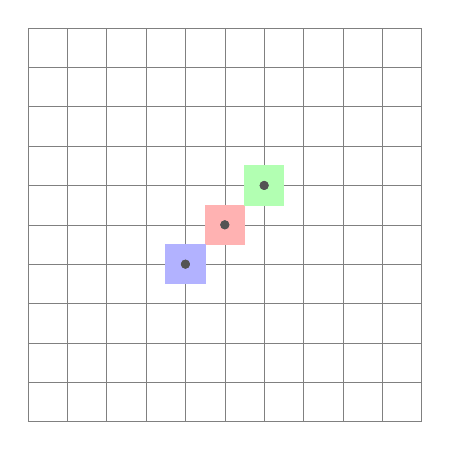
\begin{tikzpicture}[x=0.5cm,y=0.5cm]
  % colors
  \definecolor{kGreen}{rgb}{0.0,0.59,0.0}
  \definecolor{kOrange}{rgb}{1.0,0.59,0.0}
  \definecolor{kGrey}{rgb}{0.33,0.33,0.33}
  % grids
  \draw[help lines,step=0.5cm] (0,0) grid (10,10);
  % shape

  \draw[color=red!30!white,fill] (5-0.5,5-0.5) rectangle (5+0.5,5+0.5);
  \draw[color=blue!30!white,fill] (4-0.5,4-0.5) rectangle (4+0.5,4+0.5);
  \draw[color=green!30!white,fill] (6-0.5,6-0.5) rectangle (6+0.5,6+0.5);

  % gauss digitization
  \foreach \x/\y in {5/5,4/4,6/6} {
    \draw[color=kGrey,fill] (\x,\y) circle (0.5mm);
    \draw[color=kGrey,fill] (10-\x,10-\y) circle (0.5mm);
  };
\end{tikzpicture}
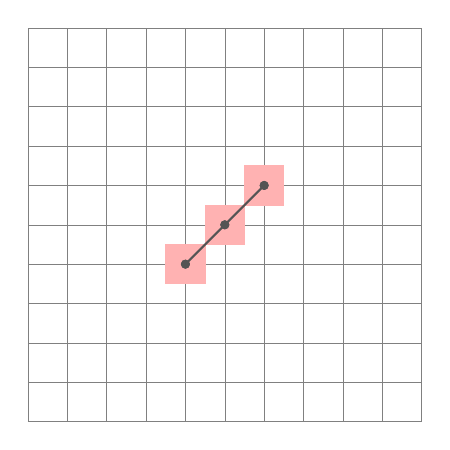
\begin{tikzpicture}[x=0.5cm,y=0.5cm]
  % colors
  \definecolor{kGreen}{rgb}{0.0,0.59,0.0}
  \definecolor{kOrange}{rgb}{1.0,0.59,0.0}
  \definecolor{kGrey}{rgb}{0.33,0.33,0.33}
  % grids
  \draw[help lines,step=0.5cm] (0,0) grid (10,10);
  % shape

  \draw[color=red!30!white,fill] (5-0.5,5-0.5) rectangle (5+0.5,5+0.5);
  \draw[color=red!30!white,fill] (4-0.5,4-0.5) rectangle (4+0.5,4+0.5);
  \draw[color=red!30!white,fill] (6-0.5,6-0.5) rectangle (6+0.5,6+0.5);

  \draw[color=kGrey,thick] (4,4) -- (5,5) -- (6,6);

  % gauss digitization
  \foreach \x/\y in {5/5,4/4,6/6} {
    \draw[color=kGrey,fill] (\x,\y) circle (0.5mm);
    \draw[color=kGrey,fill] (10-\x,10-\y) circle (0.5mm);
  };
\end{tikzpicture}

  \end{center}
  \caption[Illustration du nombre de composantes connexes en fonction de la connexité de l'espace digital.]
  %
  {Illustration du nombre de composantes connexes en fonction de la connexité de
  l'espace digital. \emph{À gauche :} trois composantes connexes sont extraites
  en $4$-connexité. \emph{À droite :} une seule composante connexe est extrait
  en $8$-connexité.\label{fig:connexite}}
  %
\end{figure}


Nous pouvons définir les \colorize{surfaces digitales}\footnote{Il existe
plusieurs définitions pour les surfaces digitales \cite{Rosenfeld1979,
Latecki1995}. Nous ne les détaillerons pas ici et n'utiliserons que la
définition la plus courante.} $\DigBoundary{\DigShape}$ comme étant le bord
topologique de l'objet digital, \cad des sous-ensemble du plan discret $\Z^n$.



En dimension 2 (\respp dimension 3), il s'agit de la région inter-pixels (\resp
inter-voxels) entre les pixels (\resp voxels) à l'intérieur de l'objet digital de
ceux à l'extérieur. Plus concrètement, les surfaces digitales sont des ensembles
de surfels et de cellules de dimensions inférieures partageant un côté à
l'intérieur de l'objet et un côté à l'extérieur (voir \cite{Herman1998,
Udupa1994, Kong1992}). La \RefFigure{fig:frontier} illustre (\emph{figure du
bas, en bleu}) le bord topologique de $\DigShape$.

% \begin{figure}[ht]
%   \begin{center}
%     
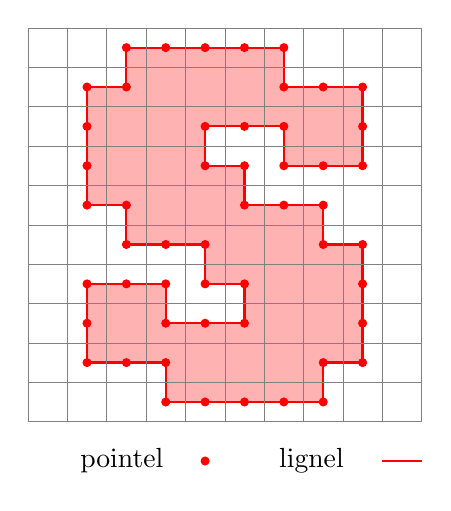
\begin{tikzpicture}[x=0.5cm,y=0.5cm]
  % colors
  \definecolor{kGreen}{rgb}{0.0,0.59,0.0}
  \definecolor{kOrange}{rgb}{1.0,0.59,0.0}
  \definecolor{kGrey}{rgb}{0.33,0.33,0.33}
  % QhZ
  \foreach \x/\y in {3/9,4/9,5/9,6/9,2/8,3/8,4/8,5/8,6/8,7/8,8/8,2/7,3/7,4/7,7/7,8/7,2/6,3/6,4/6,5/6,3/5,4/5,5/5} {
    \draw[color=red!30!white,fill] (\x-0.5,\y-0.5) rectangle (\x+0.5,\y+0.5);
    \draw[color=red!30!white,fill] (10-\x-0.5,10-\y-0.5) rectangle (10-\x+0.5,10-\y+0.5);
  };

  % pointels
  \foreach \x/\y in {1.5/1.5, 1.5/2.5, 1.5/3.5, 1.5/5.5, 1.5/6.5, 1.5/7.5, 1.5/8.5, 2.5/1.5, 2.5/3.5, 2.5/4.5, 2.5/5.5, 2.5/8.5, 2.5/9.5, 3.5/0.5, 3.5/1.5, 3.5/2.5, 3.5/3.5, 3.5/4.5, 3.5/9.5, 4.5/0.5, 4.5/2.5, 4.5/3.5, 4.5/4.5, 4.5/6.5, 4.5/7.5, 4.5/9.5}{
    \draw[color=red,fill] (\x,\y) circle (0.5mm);
    \draw[color=red,fill] (10-\x,10-\y) circle (0.5mm);
  };

  % lignels
  \draw[color=red,thick] (2.5,9.5) -- (6.5,9.5) -- (6.5,8.5) -- (8.5,8.5) -- (8.5,6.5) -- (6.5,6.5)
                             -- (6.5,7.5) -- (4.5,7.5) -- (4.5,6.5) -- (5.5,6.5) -- (5.5,5.5) -- (7.5,5.5)
                             -- (7.5,4.5) -- (8.5,4.5) -- (8.5,1.5) -- (7.5,1.5) -- (7.5,0.5) -- (3.5,0.5)
                             -- (3.5,1.5) -- (1.5,1.5) -- (1.5,3.5) -- (3.5,3.5) -- (3.5,2.5) -- (5.5,2.5)
                             -- (5.5,3.5) -- (4.5,3.5) -- (4.5,4.5) -- (2.5,4.5) -- (2.5,5.5) -- (1.5,5.5)
                             -- (1.5,8.5) -- (2.5,8.5) -- cycle;
  % grids
  \draw[help lines,step=0.5cm] (0,0) grid (10,10);
  \node at(2.5,-1) {pointel~~};
  \draw[color=red,fill] (4.5,-1) circle (0.5mm);% {\mbox{~~}};
  \node at(7.2,-1) {lignel};
  \draw[color=red,thick] (9,-1) -- (10,-1);
\end{tikzpicture}

%   \end{center}
%   \caption{Illustration du bord topologique de $\DigShape$.\label{fig:dig-boundary}}
% \end{figure}

L'autre avantage de la topologie de Khalimsky que nous pouvons exploiter est le
suivi de contour. En effet, grâce aux relations d'adjacence et à la définition
de la topologie, les algorithmes d'extraction de surface par suivi sont très
efficaces puisqu'il s'agit uniquement de résoudre un graphe de surfels.

%
\section{Discrétisation}
\label{sec:digitization}
%
Nous allons maintenant décrire le processus de discrétisation d'un sous-ensemble
de l'espace euclidien $\R^d$ vers un ensemble de points de l'espace digital
$\Z^d$. La formalisation de ce processus est importante pour l'évaluation
théorique et expérimentale des estimateurs sur les bords digitaux des objets.


Considérons une forme $\Shape$ de $\R^d$ à discrétiser en points de $\R^d$ en
coordonnées entières (\cad de $\Z^d$), alors la \colorize{discrétisation de
Gauss} $\DSh$ de $\Shape$ dans une grille de dimension $d$ et de résolution $h$
est :
%
\begin{equation}
  \DSh \EqDef \{ \vp \in \Z^d, (h \cdot \vp) \in \Shape \} \,,
\end{equation}
%
où $h \cdot \vp$ est le redimensionnement uniforme de $\vp$ par le facteur $h$.
Ce facteur $h$ est important car les points digitaux sont des carrés (ou cubes)
unitaires, et n'ont alors aucune information d'échelle permettant la
correspondance vers les forme euclidienne. Par exemple, la
\RefFigure{fig:scale-digital} montre deux disques de rayons différents
discrétisés à deux échelles $h$ différentes, donnant exactement la même
discrétisation.


\begin{figure}[ht]
  \begin{center}
    
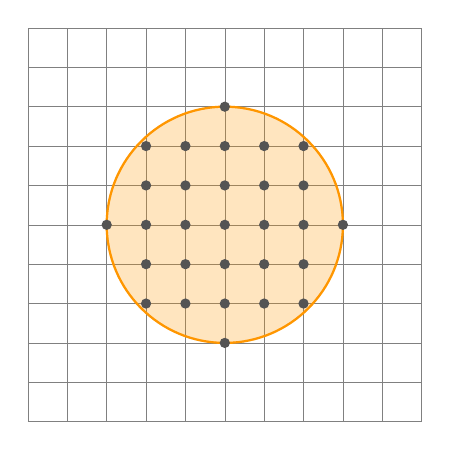
\begin{tikzpicture}[x=0.50cm,y=0.50cm]
  % colors
  \definecolor{kGreen}{rgb}{0.0,0.59,0.0}
  \definecolor{kOrange}{rgb}{1.0,0.59,0.0}
  \definecolor{kGrey}{rgb}{0.33,0.33,0.33}
  % grids
  \draw[help lines,step=1] (0,0) grid (10,10);
  \node (px) at (5,5) {};
  \draw[draw,thick,fill,color=kOrange,nearly transparent] (px) circle (3);
  \draw[draw,thick,color=kOrange] (px) circle (3);
  \foreach \x/\y in {2/5, 3/3, 3/4, 3/5, 3/6, 3/7, 4/3, 4/4, 4/5, 4/6, 4/7, 5/2, 5/3, 5/4, 5/5, 5/6, 5/7, 5/8, 6/3, 6/4, 6/5, 6/6, 6/7, 7/3, 7/4, 7/5, 7/6, 7/7, 8/5}
    \draw[draw,thick,color=kGrey,fill] (\x,\y) circle (0.1);
\end{tikzpicture}
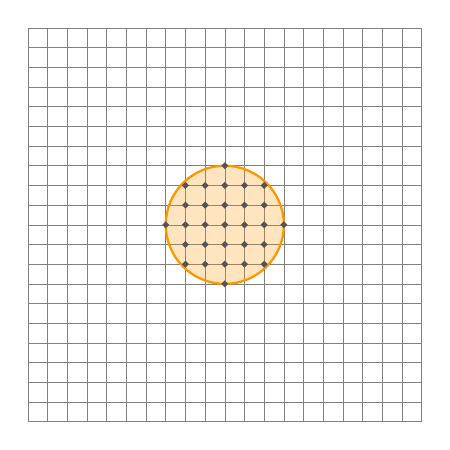
\begin{tikzpicture}[x=0.50cm,y=0.50cm]
  % colors
  \definecolor{kGreen}{rgb}{0.0,0.59,0.0}
  \definecolor{kOrange}{rgb}{1.0,0.59,0.0}
  \definecolor{kGrey}{rgb}{0.33,0.33,0.33}
  % grids
  \draw[help lines,step=0.5] (0,0) grid (10,10);
  \node (px) at (5,5) {};
  \draw[draw,thick,fill,color=kOrange,nearly transparent] (px) circle (1.5);
  \draw[draw,thick,color=kOrange] (px) circle (1.5);
  \foreach \x/\y in {3.5/5, 4/4, 4/4.5, 4/5, 4/5.5, 4/6, 4.5/4, 4.5/4.5, 4.5/5, 4.5/5.5, 4.5/6, 5/3.5, 5/4, 5/4.5, 5/5, 5/5.5, 5/6, 5/6.5, 5.5/4, 5.5/4.5, 5.5/5, 5.5/5.5, 5.5/6, 6/4, 6/4.5, 6/5, 6/5.5, 6/6, 6.5/5}
    \draw[draw,thick,color=kGrey,fill] (\x,\y) circle (0.05);
\end{tikzpicture}

  \end{center}
  \caption[Illustration de la dépendance du paramètre d'échelle $h$.]
  %
  {Illustration de la dépendance du paramètre d'échelle $h$ et de la taille de
  la forme. L'objet euclidien de gauche donne le même objet digital que l'objet
  euclidien de droite alors qu'ils sont à des échelles
  différentes.\label{fig:scale-digital}}
  %
\end{figure}

Si $\vp \in \Z^d$, alors $\Q{\vp}$ désigne le cube unitaire de dimension $d$ de
$\R^d$ centré au point $\vp$ et aligné sur les axes de $\Z^d$. Nous définissons
le \colorize{$h$-cube}, \cad $\Q{\vp}$ mis à l'échelle par $h$, comme :
%
\begin{equation}
  \hQ{\vp}{h} \EqDef h\cdot \Q{\vp} \,.
\end{equation}


Ainsi, pour un ensemble digital $\DigShape \subset \Z^d$, le
\colorize{plongement euclidien} (\anglais{body}) de $\DigShape$ est le
plongement $\Body{\cdot}{h}$ de $\DigShape$ vers $\R^d$, défini comme :
%
\begin{equation}
  \Body{\DigShape}{h} \EqDef \bigcup_{\vp \in \DigShape} \hQ{\vp}{h} \,.
\end{equation}
%
En d'autres termes, $\Body{\DigShape}{h}$ est l'ensemble des cubes de dimension
$d$ appartenant à $\DigShape$, mis à l'échelle par le pas de discrétisation $h$.


Intéressons-nous désormais aux bords de ces objets. Nous verrons plus tard que
certains estimateurs sont définis sur le bord de l'objet, il semble alors
important de l'étudier. Nous notons $\dS$ la \colorize{frontière} de $\Shape$,
\cad son bord topologique (en orange foncé sur la \RefFigure{fig:frontier}).
Nous pouvons également noter $\partial \Body{\DSh}{h}$ le bord topologique du
plongement euclidien de $\DSh$.
% La
% \colorize{$h$-frontière} $\DFr{h} \DigShape$ de l'ensemble digital $\DigShape
% \subset \Z^d$ est définie comme :
%
% \begin{equation}
  % \DFr{h} \DigShape \EqDef \partial \left( h \cdot \bigcup_{\vp \in \DigShape} \Q{\vp} \right) \,.
% \end{equation}
%


\begin{figure}[ht]
  \begin{center}
    
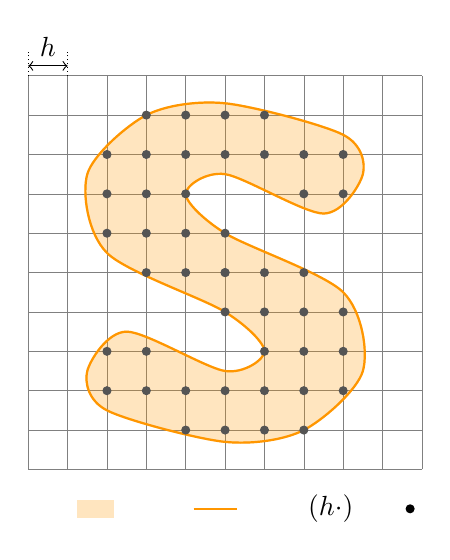
\begin{tikzpicture}[x=0.5cm,y=0.5cm]
  % colors
  \definecolor{kGreen}{rgb}{0.0,0.59,0.0}
  \definecolor{kOrange}{rgb}{1.0,0.59,0.0}
  \definecolor{kGrey}{rgb}{0.33,0.33,0.33}
  % grids
  \draw[help lines,step=0.5cm] (0,0) grid (10,10);
  % shape
  \draw[draw,thick,fill,color=kOrange,nearly transparent] plot[smooth cycle]
            coordinates{(5,9.3) (8,8.5) (8.5,7.5) (7.5,6.5) (5,7.5) (4,7) (5,6) (8,4.5) (8.5,2.5) (7,1)
                        (5,0.7) (2,1.5) (1.5,2.5) (2.5,3.5) (5,2.5) (6,3) (5,4) (2,5.5) (1.5,7.5) (3,9)} -- cycle;
  % shape boundary
  \draw[draw,thick,color=kOrange] plot[smooth cycle]
            coordinates{(5,9.3) (8,8.5) (8.5,7.5) (7.5,6.5) (5,7.5) (4,7) (5,6) (8,4.5) (8.5,2.5) (7,1)
                        (5,0.7) (2,1.5) (1.5,2.5) (2.5,3.5) (5,2.5) (6,3) (5,4) (2,5.5) (1.5,7.5) (3,9)} -- cycle;
  % gauss digitization
  \foreach \x/\y in {3/9,4/9,5/9,6/9,2/8,3/8,4/8,5/8,6/8,7/8,8/8,2/7,3/7,4/7,7/7,8/7,2/6,3/6,4/6,5/6,3/5,4/5,5/5} {
    \draw[color=kGrey,fill] (\x,\y) circle (0.5mm);
    \draw[color=kGrey,fill] (10-\x,10-\y) circle (0.5mm);
  };
  % legend
  \node at(0.5,-1) {$\Shape$};
  \node[rectangle,fill,color=kOrange,nearly transparent] at(1.7,-1) {\mbox{~~}};
  \node at(3.7,-1) {$\dS$};
  \draw[draw,thick,color=kOrange] (4.2,-1) -- (5.3,-1);
  \node at(7.8,-1) {$(h\cdot\DSh)$~~};
  \draw[color=black,fill] (9.7,-1) circle (0.5mm);
  \draw[densely dotted,black] (0,10) -- (0,10.6);
  \draw[densely dotted,black] (1,10) -- (1,10.6);
  \draw[<->,black] (0,10.25) -- (1,10.25) node[midway,above] {$h$};
\end{tikzpicture}
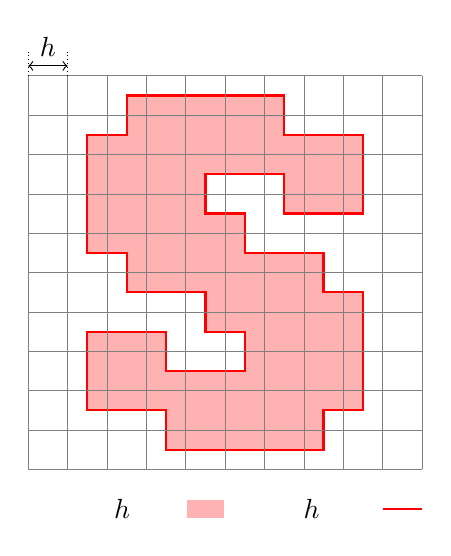
\begin{tikzpicture}[x=0.5cm,y=0.5cm]
  % colors
  \definecolor{kGreen}{rgb}{0.0,0.59,0.0}
  \definecolor{kOrange}{rgb}{1.0,0.59,0.0}
  \definecolor{kGrey}{rgb}{0.33,0.33,0.33}
  % QhZ
  \foreach \x/\y in {3/9,4/9,5/9,6/9,2/8,3/8,4/8,5/8,6/8,7/8,8/8,2/7,3/7,4/7,7/7,8/7,2/6,3/6,4/6,5/6,3/5,4/5,5/5} {
    \draw[color=red!30!white,fill] (\x-0.5,\y-0.5) rectangle (\x+0.5,\y+0.5);
    \draw[color=red!30!white,fill] (10-\x-0.5,10-\y-0.5) rectangle (10-\x+0.5,10-\y+0.5);
  };
  % \partial_h X
  \draw[color=red,thick] (2.5,9.5) -- (6.5,9.5) -- (6.5,8.5) -- (8.5,8.5) -- (8.5,6.5) -- (6.5,6.5)
                             -- (6.5,7.5) -- (4.5,7.5) -- (4.5,6.5) -- (5.5,6.5) -- (5.5,5.5) -- (7.5,5.5)
                             -- (7.5,4.5) -- (8.5,4.5) -- (8.5,1.5) -- (7.5,1.5) -- (7.5,0.5) -- (3.5,0.5)
                             -- (3.5,1.5) -- (1.5,1.5) -- (1.5,3.5) -- (3.5,3.5) -- (3.5,2.5) -- (5.5,2.5)
                             -- (5.5,3.5) -- (4.5,3.5) -- (4.5,4.5) -- (2.5,4.5) -- (2.5,5.5) -- (1.5,5.5)
                             -- (1.5,8.5) -- (2.5,8.5) -- cycle;
  % grids
  \draw[help lines,step=0.5cm] (0,0) grid (10,10);
  \node at(2.5,-1) {$\Body{\DSh}{h}$~~};
  \node[color=red!30!white,fill] at(4.5,-1) {\mbox{~~}};
  \node at(7.2,-1) {$\Bd{\Body{\DSh}{h}}$}; %% := \partial \hCube{h} \GD{h}X$};
  \draw[color=red,thick] (9,-1) -- (10,-1);
  \draw[densely dotted,black] (0,10) -- (0,10.6);
  \draw[densely dotted,black] (1,10) -- (1,10.6);
  \draw[<->,black] (0,10.25) -- (1,10.25) node[midway,above] {$h$};
\end{tikzpicture}

  \end{center}
  %
  \caption{\emph{De gauche à droite en haut :} Illustration d'une forme
  euclidienne $\Shape$ (\emph{en orange pâle}), de sa frontière $\dS$ (\emph{en
  orange foncé}), du plongement euclidien de sa discrétisation de Gauss
  $\Body{\DSh}{h}$ (\emph{en rouge pâle}) et son bord topologique euclidien
  $\partial\Body{\DSh}{h}$ (\emph{en orange foncé}). \emph{En bas :} l'objet
  digital $\DigShape = \DSh$ (\emph{en gris}, à noter que les carrés de la
  grille sont unitaires) et son bord digital $\DigBoundary{\DSh}$ (\emph{en
  bleu}) composé de lignels et pointels. \label{fig:frontier}}
  %
\end{figure}


La \RefFigure{fig:frontier} montre une forme euclidienne $\Shape \subset \R^2$
(en orange pâle) et sa frontière $\dS$ (en orange foncé), ainsi que
$\Body{\DSh}{h}$ le plongement euclidien de la discrétisation de Gauss de
$\Shape$ avec le pas de discrétisation $h$ (en rouge pâle) et son bord euclidien
$\partial\Body{\DSh}{h}$ (en rouge foncé). La figure du bas de la
\RefFigureN{fig:frontier} montre l'objet digital $\DigShape$ ($= \DSh$) que nous
obtenons après la discrétisation de $\Shape$ dans l'espace de Khalimsky au pas
de discrétisation $h$ (en gris). Ainsi, nous obtenons des points digitaux $\vp
\in \Z^2$ dans une grille carré régulière unitaire. Nous pouvons extraire le
bord $\DigBoundary{\DigShape}$ afin d'obtenir un ensemble de lignels et de
pointels (en bleu).


Comme nous pouvons le voir sur la \RefFigure{fig:frontier}, la bord
$\partial\Body{\DSh}{h}$ du plongement euclidien de $\DSh$ est un sous-ensemble
de dimension $(d-1)$ de $\R^d$ qui est proche de $\partial \Shape$. Pour
certaines preuves mathématiques cette notion de proximité est essentielle. Une
correspondance précise entre les points $\vx \in \dS$ et $\hat{\vx}\in
\partial\Body{\DSh}{h}$ est alors nécessaire. Définissons dans un premier temps
les outils dont nous avons besoin pour étudier cette correspondance : pour un
forme $\Shape \subset \R^d$, l'\colorize{axe médian} $MA(\dS)$ de $\dS$ est le
sous-ensemble de $\R^d$ dans lequel chacun des points est le plus proche d'au
moins deux points de $\dS$. Le \colorize{reach} de $\dS$ est la borne
inférieure de la distance entre $\dS$ et son axe médian. Les formes à reach
positif ont leur courbures principales bornées par $\pm 1 / \Reach{\Shape}$.
% Nous définissons la \colorize{projection orthogonale} $\ProjX{\Shape}$ comme la
% correspondance de $\Shape \setminus MA(\dS)$ vers $\dS$ qui associe tout point
% vers son point le plus proche de $\dS$.
%
% \\
%
Alors nous pouvons définir la correspondance $\Proj$ du bord
$\partial\Body{\DSh}{h}$ du plongement euclidien de la discrétisation de Gauss
de $\Shape$ vers le bord topologique $\dS$ de $\Shape$ dans la direction de la
normale de la surface. Cette projection est nommée la \colorize{projection
inverse} ou \anglais{back-projection} \cite{Lachaud2006HDR} :
%
\begin{definition}{\fakeTitle{Projection inverse $\Proj$ \cite{Lachaud2006HDR}}}
\label{def:projection}
%
  Pour tout forme 2D $\Shape$ à reach positif, pour $0 < h \le \Reach{\Shape}$,
  soit $\NormalDir(\Shape,\vx,l)$ le segment centré au point $\vx$, aligné le
  long de la normale au point $\vx$ et de demi-longueur $l$ Alors la
  \colorize{projection inverse} $\Proj$ est définie comme :
  %
  \begin{align}
    \Proj: \partial\Body{\DigShape}{h} &\rightarrow \dS, \nonumber \\
    \hat{\vx} &\mapsto \vx=\Proj(\hat{\vx}) \,,
  \end{align}
  %
  où $\vx$ est le seul point tel que $\hat{\vx} \in
  \NormalDir(\Shape,\vx,\frac{\sqrt{2}}{2}h)$.
%
\end{definition}
%
Le \RefLemmaFake{B.9}{Lachaud2006HDR} nous indique que la correspondance $\Proj$
n'introduit aucune ambiguïté et est surjectif si $h < h_0$ et si le bord de
$\Shape$ est $C^3$-convexe, et le \RefLemmaFake{B.10}{Lachaud2006HDR} que cette
correspondance est continue. La \RefFigure{fig:backproj} nous montre (en rouge)
la projection de tout point $\hat{\vx} \in \partial\Body{\DSh}{h}$ vers des
points $\vx \in \dS$. Alors, nous pouvons conclure que les bords
$\partial\Body{\DSh}{h}$ et $\dS$ ont une distance de Hausdorff inférieure ou
égale à $\frac{\sqrt{2}}{2}h$. De plus, la projection $\ProjX{\Shape}$ est
continue sur $\R^d \setminus MA(\dS)$, donc également sur
$\partial\Body{\DSh}{h}$ avec un $h$ adéquat. En dimension supérieure, nous
pouvons citer les travaux de \cauthors{Lachaud}{Lachaud2015}, qui mettent aussi
en évidence l'équivalence des notions de reach et de
par($R$)-régularité\footnote{correspond à des formes dont les normales ne
s'intersectent pas entre elles lorsqu'elles sont représentés comme des segments
de longueurs $2R$}.


\begin{figure}[t]{\small
    \begin{center}
      {\begin{overpic}[width=8cm]{images/Notions/notation}
          \put(43,23.5){$\hat{\vx}$}
          \put(41,29){$\vx$}
          \put(39,15){$h$}
          \put(77,39){$\Proj(\hat{\vx})$}
          \put(5,15){$\dS$}
          \put(17,10){$\partial\Body{\DSh}{h}$}
      \end{overpic}}
    \end{center}}
    \caption{Projection inverse de tout point $\hat{\vx} \in \partial\Body{\DSh}{h}$ vers des
    points $\vx \in \dS$.\label{fig:backproj}}
\end{figure}
%
\section{Convergence asymptotique d'estimateurs locaux et globaux}
\label{sec:multigrid-convergence-estimator}
%
Maintenant que le processus de discrétisation est défini, nous allons nous
intéresser aux propriétés de convergence asymptotique des estimateurs de
quantités géométriques. Tout d'abord, nous pouvons distinguer deux types de
quantités géométriques : les quantités « locales » et les quantités « globales » :
%
\begin{definition}{\fakeTitle{Quantités géométriques locales et globales}}
  \label{def:global-quantity}
  %
  Une quantité géométrique est dite « locale » lorsqu'elle est définie
  localement sur le bord de la forme. Une quantité géométrique est dite «
  globale » lorsqu'elle est associée à la forme toute entière.
  %
\end{definition}
%
Il apparaît alors clairement que, par exemple, le volume d'une forme est une
quantité géométrique « globale », tandis que la normale, la courbure ou encore
la tangente en un point de sa surface sont des quantités géométriques dites « locales ».


Nous allons désormais définir la \colorize{convergence asymptotique
d'estimateurs} de quantités géométriques (locales et globales). La notion de
convergence asymptotique, introduite en $1982$ par \cauthor{Serra}{Serra1982},
est un critère important permettant d'évaluer et de comparer des estimateurs
digitaux. L'idée principale est, pour une forme euclidienne $\Shape$ donnée,
d'évaluer l'erreur entre une quantité géométrique de $\Shape$ et la quantité
géométrique digitale estimée sur la discrétisation de $\Shape$, à plusieurs
échelles de discrétisation. Le comportement attendu est alors que si nous
raffinons l'objet digital (\cad que le pas de discrétisation diminue, donnant
ainsi un objet digital plus proche de la forme euclidienne comme le montre la
\RefFigure{fig:digital-ellipse}), l'erreur d'estimation doit tendre vers $0$.


\begin{figure}[ht]{
    \begin{center}
    %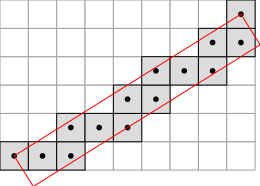
\includegraphics[width=6cm]{images/Notions/StandardDSS4bis}
    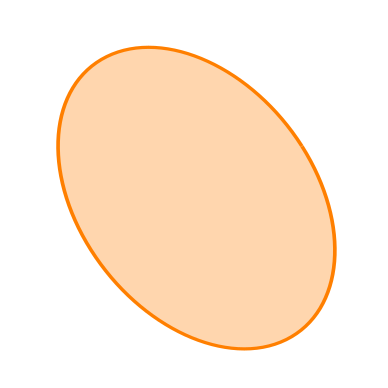
\includegraphics[width=3.4cm]{images/Notions/multi-ellipse-0}
    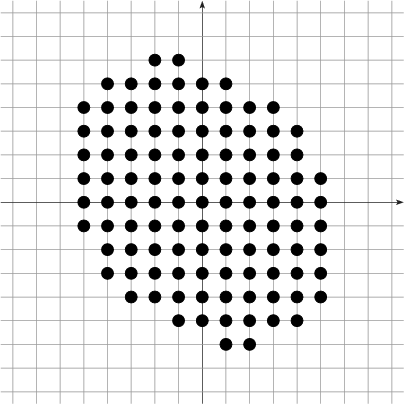
\includegraphics[width=3.4cm]{images/Notions/multi-ellipse-1}
    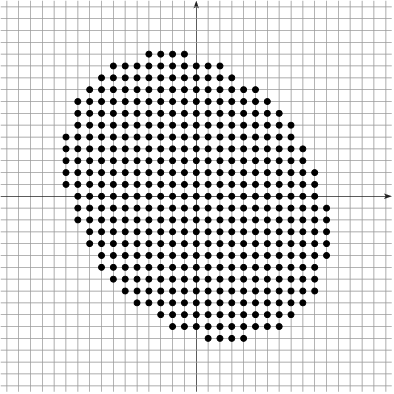
\includegraphics[width=3.4cm]{images/Notions/multi-ellipse-2}
    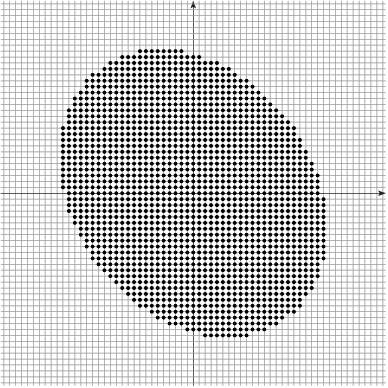
\includegraphics[width=3.4cm]{images/Notions/multi-ellipse-4}
    \end{center}}
    \caption{Ellipse euclidienne et ses versions discrétisées à différents pas de discrétisation $h = 1$, $0.5$ et $0.1$.\label{fig:digital-ellipse}}
\end{figure}


Ainsi, définissons $\hat{E}(\DSh,h)$ (\respp $\hat{E}(\DSh,\hat{\vx},h)$) un
estimateur de quantité géométrique globale (\resp locale) sur $\DSh$ la
discrétisation (de Gauss, voir le \RefSection{sec:digitization}) de la forme
$\Shape$ au pas de discrétisation $h$. La version locale est définie sur un
point $\hat{\vx}$ le bord digital $\partial\Body{\DSh}{h}$ de la discrétisation
de la forme $\Shape$ au pas de discrétisation $h$.


Alors, nous pouvons étudier la convergence asymptotique de ces estimateurs
(issue de la \RefDefinitionFake{2.10}{Klette2004}) :
%
\begin{definition}{\fakeTitle{Convergence asymptotique d'un estimateur digital de quantité géométrique globale}}
  \label{def:multigrid-convergence-global}
  %
  Un estimateur digital de quantité géométrique globale $\hat{E}$ d'une quantité géométrique
  $E$ \colorize{converge asymptotiquement} pour une famille de formes $\Shapes$ si
  et seulement si pour toute forme $\Shape \in \Shapes$, il existe un pas de
  discrétisation $h_0 > 0$ tel que l'estimation de $\hat{E}(\DSh,h)$
  soit défini pour tout $0 < h < h_0$,
  %
  \begin{equation}
    | \hat{E}(\DSh,h) - E(\Shape) | \le \tau_{\Shape}(h) \,,
  \end{equation}
  %
  où $\tau_{\Shape}: \R^{+*} \rightarrow \R^+$, désignant l'erreur d'estimation
  de la quantité géométrique pour le pas de discrétisation $h$, a une limite
  nulle à $0$. Cette fonction définie la vitesse de convergence de $\hat{E}$
  vers $E$ sur $\Shape$.
  %
\end{definition}
%
% Lorsqu'une quantité géométrique est « locale », nous avons besoin de la
% propriété de projection inverse (\RefDefinition{def:projection}) afin de
% connaître explicitement la correspondance entre $\dS$ et le bord du plongement
% euclidien de sa discrétisation $\partial\Body{\DSh}{h}$.
%
Un estimateur local digital estime la quantité géométrique sur tout point
$\hat{\vx}$ de $\partial\Body{\DSh}{h}$.
%
\begin{definition}{\fakeTitle{Convergence asymptotique d'un estimateur digital de quantité géométrique locale}}
  \label{def:multigrid-convergence-local}
  %
  Un estimateur digital de quantité géométrique locale $\hat{E}$ d'une quantité géométrique
  $E$ \colorize{converge asymptotiquement} pour une famille de formes $\Shapes$ si
  et seulement si pour toute forme $\Shape \in \Shapes$, il existe un pas de
  discrétisation $h_0 > 0$ tel que l'estimation de $\hat{E}(\DSh,\hat{\vx},h)$
  soit défini en tout point $\hat{\vx} \in \partial \Body{\DSh}{h}$ avec $0 < h < h_0$,
  et pour tout $\vx \in \dS$,
  %
  \begin{equation}
    \forall \hat{\vx} \in \partial\Body{\DSh}{h} \text{~avec~} \| \hat{\vx} -\vx\|_\infty
    \le h, \quad | \hat{E}(\DSh,\hat{\vx},h) - E(\Shape,\vx) | \le \tau_{\Shape,\vx}(h) \,,
  \end{equation}
  %
  où $\tau_{\Shape,\vx}: \R^{+*} \rightarrow \R^+$ a une limite
  nulle à $0$. Cette fonction définie la vitesse de convergence de $\hat{E}$
  vers $E$ au point $\vx$ de $\Shape$. La convergence est dite
  \colorize{uniforme} pour $\Shape$ lorsque toutes les valeurs de
  $\tau_{\Shape,\vx}$ sont bornées (borne supérieure) par une fonction
  $\tau_\Shape$ indépendante de $\vx \in \dS$ avec une limite nulle à $0$.
  %
\end{definition}

Lorsque nous implémentons un estimateur différentiel sur une surface digitale,
l'estimation est donnée sur un élément de la surface combinatoire (une surfel ou
un élément de dimension inférieure). Implicitement, nous estimons en un point
$\hat{\vx}$ correspondant au centre du plongement géométrique du surfel. Nos
preuves de convergences étant définies pour tout $\hat{\vx}$ de $\partial
\Body{\DSh}{h}$, ce type d'implémentation des estimateurs digitaux reste
parfaitement cohérent.

Généralement, les vitesses de convergence des estimateurs étudiés seront de la
forme $O(h^a)$, pour $a > 0$ et $h$ qui tend vers $0$. Cette valeur de $a$ nous
permet alors de comparer les vitesses de convergence des estimateurs. Nous nous
intéressons dans cette thèse à la \colorize{convergence asymptotique uniforme}
de nos estimateurs, en d'autres mots il s'agit l'erreur dans le pire des cas de
nos estimateurs.

Les preuves de convergences sont valides seulement pour des \colorize{familles d'objets}
$\Shapes$. Ces familles d'objets font des hypothèses sur la formes, permettant
alors de valider la convergence.
\begin{itemize}
  \item La famille de toutes les formes convexes finies du plan euclidien est noté $\Shape^{C}$;
  \item La famille de tous les ensembles convexes dont la bordure est $C^n$ à courbure positive est noté $\Shape^{n-SC}$;
  \item La famille de tous les ensembles convexes dont la bordure est $C^n$ par morceaux est noté $\Shape^{n-PW-SC}$.
\end{itemize}
%
%\subsection{Tableau récapitulatif de convergence d'estimateurs de quantités géométriques}
%

\cauthors{Coeurjolly}{Coeurjolly_ChapEstimateur} ont proposé une analyse
complète d'estimateurs (en dimension 2) de la longueur de la forme (ou
périmètre) ainsi que de la tangente en tout point du bord de l'objet. Le
\RefTable{tab:tang-comp} récapitule les vitesses de convergence obtenues ainsi
que les familles de formes associées pour les preuves de convergence.
L'estimation de la courbure sera détaillée dans le chapitre suivant.


\begin{table}[ht]
\centering
\caption{Convergence asymptotique connus de certains estimateurs de quantités géométriques (\RefTablesFake{1}{2}{Coeurjolly_ChapEstimateur}).}
\label{tab:tang-comp}
\begin{tabular}{@{}lp{1.9cm}lllr@{}}
\toprule
 & & & \multicolumn{2}{c}{Vitesse de convergence} &            \\ \cmidrule(r){4-5}
Quantité & Estimateur & Famille de formes & Borne sup. & Observée & Référence \\ \midrule

% Aire & $\AreaC$ & $\Shapes^{C}$ & $O(h)$ & & \cite{Klette2000} \\
% Aire & $\AreaC$ & $\Shapes^{3-PW-SC}$ & $O(h^{\frac{15}{11} + \epsilon})$ & & \cite{Huxley1990} \\
%
% Volume & $\VolC$ & $\Shapes^{3-PW-SC}$ & $O(h)$ & & \cite{} \\
% Volume & $\VolC$ & $\Shapes^{3-SC}$ & $O(h)$ & & \cite{} \\
Longueur & $\hat{\vL}^{DSS}$ & Polygones convexes & $\approx 4.5h$ & & \cite{Kovalevsky1992} \\
Longueur & $\hat{\vL}^{DSS}$ & $\Shapes^{3-PW-SC}$ & ? & $O(h)$ & \cite{Kovalevsky1992} \\
Longueur & $\epsilon-sausage$ & Polygones convexes & $\approx 5.844h$ & & \cite{Asano2001} \\
Longueur & $\hat{\vL}^{ST}$ & $\Shapes^{C}$ & ? & $O(h)$ & \cite{Coeurjolly2004} \\
Longueur & $\hat{\vL}^{FP}$ & $\Shapes^{C}$ & ? & $O(h)$ & \cite{Roussillon2011b} \\
Longueur & $\hat{\vL}^{MLP}$ & $\Shapes^{C}$ & $\approx 8h$ & & \cite{Sloboda1998} \\
Longueur & $\hat{\vL}^{MLP}$ & $\Shapes^{3-PW-SC}$ & $O(h)$ & $O(h^\frac{4}{3})$ & \cite{Sloboda1998} \\
Longueur & $\hat{\vL}^{\lambda-MST}$ & $\Shapes^{3-PW-SC}$ & $O(h^\frac{1}{3})$ & $O(h^\frac{4}{3})$ & \cite{Lachaud2006HDR} \\

Tangente & $\hat{\vT}^{BC}$ & Polygones & ? & $O(h^\frac{1}{3})$ & \cite{Coeurjolly_ChapEstimateur} \\
Tangente & $\hat{\vT}^{BC}$ & $\Shapes^{1-SC}$ & $O(h^\frac{2}{3})$ & $O(h^\frac{2}{3})$ & \cite{Malgouyres2008} \\
Tangente & $\hat{\vT}^{BC}$ & $\Shapes^{1-PW-SC}$ & ? & $O(h^\frac{1}{3})$ & \cite{Coeurjolly_ChapEstimateur} \\

Tangente & $\hat{\vT}^{\lambda-MST}$ et $\hat{\vT}^{MCMS}$ & Polygones & $O(h)$ & $O(h)$ & \cite{Lachaud2006HDR} \\
Tangente & $\hat{\vT}^{\lambda-MST}$ et $\hat{\vT}^{MCMS}$ & $\Shapes^{1-PW-SC}$ & ? & $O(h^\frac{2}{3})$ & \cite{deVieilleville2009} \\
Tangente & $\hat{\vT}^{\lambda-MST}$ et $\hat{\vT}^{MCMS}$ & $\Shapes^{3-SC}$ & $O(h^\frac{1}{3})$ & $O(h^\frac{2}{3})$ & \cite{Lachaud2006HDR} \\

Tangente & $\hat{\vT}^{H1-0GD}$ & Polygones & ? & \svgNope & \cite{Coeurjolly_ChapEstimateur} \\
Tangente & $\hat{\vT}^{H1-0GD}$ & $\Shapes^{1-PW-SC}$ & ? & $\approx O(h^\frac{2.5}{3})$ & \cite{deVieilleville2009} \\
Tangente & $\hat{\vT}^{H1-0GD}$ & $\Shapes^{3-SC}$ & $O(h^\frac{1}{3})$ & $O(h^\frac{2.5}{3})$ & \cite{deVieilleville2009} \\

\bottomrule
\end{tabular}
\end{table}

Pour plus de détails, se référer à \cite{Coeurjolly_ChapEstimateur}. La
convergence des estimateurs de courbure sera détaillé dans le chapitre suivant.
Intéressons-nous dans le paragraphe suivant à l'estimation de l'aire, du volume
et des moments géométriques.
%
\section{Estimateurs digitaux d'aire, de volume, de moments géométriques}
\label{sec:aire-volume-moments}
%
Nous avons vu dans le \RefSection{sec:geo-diff} certaines quantités
intégrales, comme l'aire, le volume ou encore les moments. Ces quantités
peuvent être très facilement estimées sur des surfaces
digitales, le calcul intégral pouvant se limiter à compter des points digitaux.
Nous allons ici détailler l'estimation digitale d'aire, de volume et des moments
sur des surfaces digitales, ainsi que leurs convergences.
%
\subsection{Aire et volume digitaux en dénombrant les points digitaux}
\label{sec:AreaByCounting}
%
Une façon simple de calculer l'aire ou le volume d'une forme digitale consiste à
compter le nombre de points digitaux appartenant à la forme. Plus formellement,
pour tout sous-ensemble $\DigShape \subset \Z^2$, l'estimateur digital d'aire au pas
de discrétisation $h$ est défini par :
%
\begin{equation}
  \AreaC(\DigShape, h) \EqDef h^2 \MCard(\DigShape)
\end{equation}
%
En dimension $3$, nous noterons ainsi l'estimateur digital de volume au pas de
discrétisation $h$ :
%
\begin{equation}
  \VolC(\DigShape, h) \EqDef h^3 \MCard(\DigShape)
\end{equation}
%
Maintenant, si ce sous-ensemble digital $\DigShape$ provient de la discrétisation de
formes euclidiennes $\Shape$, nous voulons que l'estimation du volume devienne
meilleure lorsque le pas de discrétisation $h$ se raffine (voir
\RefSection{sec:multigrid-convergence-estimator}). Il est connu depuis
\nauthor{Gauss} et \nauthor{Dirichlet} que cette façon d'estimer l'aire donne
des résultats de convergence asymptotique sur les formes $\Shape$ convexes
finies de $\R^2$ :
%
\begin{equation}
  \label{eq:AreaByCountingConv}
  \AreaC(\DigF{\Shape}{h},h) = \Area(\Shape) + O(h^\beta),
\end{equation}
%
avec $\beta = 1$ dans le cas général ($\Shapes^{C}$) \cite{Klette2000}, et peut être optimisé à
$\beta = \frac{15}{11} - \epsilon$ avec $\epsilon > 0$ (arbitrairement petit)
lorsque le bord de l'objet est $C^3$ à courbure non nulle \cite{Huxley1990}.
De mêmes résultats ont été proposés en 3D :
%
\begin{equation}
  \label{eq:VolumeByCountingConv}
  \VolC(\DigF{\Shape}{h},h) = \Vol(\Shape) + O(h^\gamma),
\end{equation}
%
avec $\gamma = 1$ dans le cas général \cite{Kratzel1988}, et peut être amélioré à
$\gamma=\frac{243}{158}$ lorsque le bord est lisse ($\Shapes^{3-SC}$) \cite{Guo2010}.
%
En dimension 2, les objets non convexes suivent les mêmes règles tant que
$\Shape$ peut être exprimé comme une somme ou une différence de régions convexes
bornées par des courbes fermées simples \cite{Huxley1996}. Ces résultats
précédents restent valides chaque fois que le bord de la forme peut être
décomposé en nombre fini de morceaux convexes (ou convexe $C^3$ à courbure non
nulle pour les bornes améliorées).
%
\subsection{Moments géométriques digitaux en dénombrant les points digitaux}
\label{sec:MomentsByCounting}
%
Comme pour l'aire ou le volume précédemment, il est très simple de calculer les
moments sur des données digitales. En effet, il suffit de sommer les valeurs des
points digitaux de la forme et de remettre à l'échelle suivant le pas de
discrétisation $h$. Plus formellement, pour tout sous-ensemble $\DigShape$ de
$\Z^d$, le $p_1 \cdots p_d$-moment digital de $\DigShape$ au pas de
discrétisation $h$ est défini par :
%
\begin{equation} \label{eq:MomentsByCounting-def}
%
  \DMom{p_1 \cdots p_d}{h}(\DigShape) \EqDef h^{d + p_1 + \cdots + p_d} \sum_{(z_1,\ldots,z_d) \in \DigShape} z_1^{p_1} \cdots z_d^{p_d} \,.
%
\end{equation}
%
Ainsi, le $0$-moment digital de $\DigShape$ correspond au volume digital de
$\DigShape$, \cad $\AreaC(\DigShape,h)$ lorsque $d = 2$ et $\VolC(\DigShape,h)$
lorsque $d \geq 3$.
%
Nous souhaitons alors borner l'erreur entre les moments de $\Shape$ et
l'estimation des moments digitaux de la discrétisation de $\Shape$ comme
fonction du pas de discrétisation $h$. \cauthors{Klette}{Klette2000} ont
démontré la convergence de cet estimation des moments avec une vitesse de
convergence dépendante de l'ordre du moment $\sigma = p_1 + \cdots + p_d$ :
%
\begin{equation} \label{eq:MomentsByCounting-conv}
%
  \DMom{p_1 \cdots p_d}{h}(\DigF{\Shape}{h},h) = \Mom{p_1 \cdots p_d}(\Shape) + O(h^{\mu_{\sigma}}).
%
\end{equation}
%
avec $\mu_{\sigma} \ge 1$ en dimension 2 et 3, pour $\sigma \le 2$.
%(\todoJeremy{expliciter}).
Cette borne peut être améliorer lorsque la courbure gaussienne n'est pas nulle :
\cauthors{Krätzel}{Kratzel1991} obtiennent $\mu_0=\frac{38}{25}-\epsilon$ et
\cauthors{Müller}{Muller1999} obtiennent $\mu_0 = \frac{66}{43}-\epsilon$.
%
\section{Droites digitales standards, segments digitaux, arcs de cercle digitaux}%
\label{sec:segments}
%
Nous allons maintenant nous intéresser aux définitions de primitives digitales.
La primitive la plus basique à reconnaître est sans nul doute la droite ou le
segment de droite. Alors nous devons définir ce qu'une droite représente dans
l'espace digital et ce n'est pas trivial à cause de la discrétisation de la
forme. Définissons tout d'abord une \colorize{droite digitale standard} (ou
droite $4$-connexe), et ainsi le \colorize{segment digital} (voir la
\RefFigure{fig:dss-figure}) :
%
\begin{definition}{\fakeTitle{Droite digitale standard et segment digital (« \anglais{Standard Digital Straight Segment} ») \cite{Reveilles1991}}}
  \label{def:DSS}
%
  L'ensemble de points $(p_1,p_2) \in \Z^2$ satisfaisant $\mu \le ap_1 - bp_2 <
  \mu + |a| + |b|$, avec $a$, $b$ et $\mu$ des nombres entiers, est appelé une
  \colorize{droite digitale standard} avec comme pente $a/b$ et comme décalage
  $\mu$. Tout sous ensemble de pixels connectés d'une droite digitale standard
  est un \colorize{segment digital} (ou « \anglais{DSS} »).
%
\end{definition}
%
Cette droite est $4$-connexe, et en fait un candidat parfait pour être reconnu à
partir d'un contour digital.

\begin{figure}[ht]{
    \begin{center}
    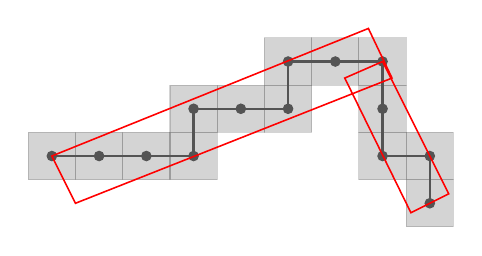
\begin{tikzpicture}[x=0.6cm,y=0.6cm]
  \definecolor{kGrey}{rgb}{0.33,0.33,0.33}

  \foreach \x/\y in { 0/0,1/0,2/0,3/0,3/1,4/1,5/1,5/2,6/2,7/2,7/1,7/0,8/0,8/-1 }
  {
    \draw[color=kGrey,fill, nearly transparent] (\x-0.5,\y-0.5) rectangle (\x+0.5,\y+0.5);
    \draw[color=kGrey,fill] (\x,\y) circle (0.1);
  }

  \draw[color=kGrey,thick] (0,0) -- (3,0) -- (3,1) -- (5,1) -- (5,2) -- (7,2) -- (7,0) -- (8,0) -- (8,-1);

  \draw[color=red,line width=0.2mm] (0,0) -- (6.7,2.7) -- (7.2,1.65) -- (0.5,-1) -- cycle;
  \draw[color=red,line width=0.2mm] (7,2) -- (8.4,-0.8) -- (7.6,-1.2) -- (6.2,1.65) -- cycle;
\end{tikzpicture}\quad

    \end{center}}
    \caption{Segments de droites digitales (en rouge sur la figure).\label{fig:dss-figure}}
\end{figure}

% et étudier estimées et, grâce à leurs bonnes propriétés
% mathématiques, pourront utilisées par la suite comme point d'entré d'estimateurs
% de quantités différentielles comme la courbure (ce que nous verrons dans le
% \RefChapitre{sec:estimators}).

Nous pouvons alors faire de la reconnaissance de ces primitives. La définition
suivante décrit la manière de reconnaître un \colorize{segment maximal} à partir
d'un ensemble de points digitaux, ainsi que le \colorize{faisceau de segments
maximaux} :
%
\begin{definition}{\fakeTitle{Segments maximaux et faisceau de segments maximaux \cite{Lachaud2007}}}
  \label{def:MDSS}
%
  Les pointels composant le bord digital $\BdZ{\DigShape}$ d'une forme
  $\DigShape \subset \Z^2$ forment un contour $4$-connecté. Cela nous permet de
  les dénombrer consécutivement par $(\vp_i)_{i={0\ldots n-1}}$. Une séquence de
  pointels $(\vp_i, \ldots, \vp_j)$ (dont l'indice est modulo $n$) est un
  \colorize{segment maximal} (ou « \anglais{MDSS} ») sur $\BdZ{\DigShape}$ si c'est
  un DSS qui ne peut s'étendre dans aucun sens (en avant ou en arrière) en
  restant un DSS.
  %
  \\
  %
  Plus formellement, $(\vp_i, \ldots, \vp_j)$ est un segment maximal sur $\BdZ{\DigShape}$ \ssi :
  \begin{itemize}
    \item $(\vp_i, \ldots, \vp_j)$ est un DSS sur $\BdZ{\DigShape}$,
    \item $(\vp_{i-1}, \ldots, \vp_j)$ n'est pas un DSS sur $\BdZ{\DigShape}$,
    \item $(\vp_i, \ldots, \vp_{j+1})$ n'est pas un DSS sur $\BdZ{\DigShape}$,
  \end{itemize}
  %
  Pour un pointel $\vp \in \BdZ{\DigShape}$ donné, le \emph{faisceau de segments maximaux} à $\vp$ est l'ensemble
  des segments maximaux de $\BdZ{\DigShape}$ contenant $\vp$.
%
\end{definition}


Il parait alors essentiel d'étudier le comportement asymptotique de ces
primitives afin de pouvoir les exploiter au sein d'estimateurs auxquels nous
voulons prouver la convergence. \cauthors{Lachaud}{Lachaud2006HDR} et
\cauthors{de Vieilleville}{deVieilleville2007} se sont alors intéressés aux
propriétés asymptotiques des longueurs des segments maximaux sur des formes
convexe suffisamment lisse de dimension $2$ :
%
\begin{lemma}{\fakeTitle{Lois asymptotiques des segments maximaux}}
  \label{lem:law-length-MDSS}
  %
  Soit $\Shape$ une forme convexe de $\R^2$, avec un bord $C^3$ à
  courbure bornée non nulle. La longueur discrète des segments maximaux de
  $\BdZ{\DigShape}$ pour $\DigShape = \DSh$ suit les règles suivantes :
  %
  \begin{itemize}
    %
    \item le \colorize{plus court des segments maximaux} a une borne inférieure en
    $\Omega(h^{-\frac{1}{3}})$;
    %
    \item le \colorize{plus long des segments maximaux} a une borne supérieure en
    $O(h^{-\frac{1}{2}})$;
    %
    \item la \colorize{longueur moyenne des segments maximaux} $L_D({\DigShape})$, est
    bornée par :
    %
    \begin{equation}
      \label{eq:lengthMS}
      \Theta(h^{-\frac{1}{3}}) \le L_D( {\DigShape} ) \le \Theta(h^{-\frac{1}{3}} \log \left(\frac{1}{h}\right))\;.
    \end{equation}
  \end{itemize}
  %
\end{lemma}


\begin{figure}[ht]{
    \begin{center}
    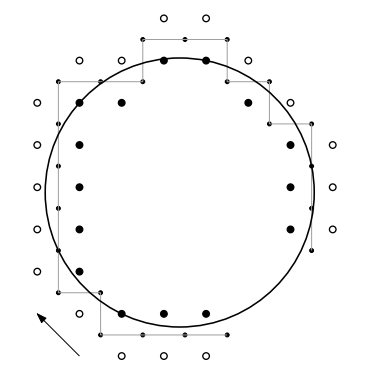
\includegraphics[height=6cm]{images/Notions/DCA}
    \end{center}}
    \caption[Arc de cercle digital.]{Arc de cercle digital (Figure~1.22 de \cite{Roussillon2009}).\label{fig:dca-figure}}
\end{figure}


L'arc de cercle est une autre primitive intéressante à étudier. En effet,
puisque la courbure est l'inverse du rayon du cercle osculateur du bord d'un
objet, le reconnaître permettrait d'approcher cette valeur. Définissons alors
\colorize{l'arc de cercle digital} (voir la \RefFigure{fig:dca-figure}) :
%
\begin{definition}{\fakeTitle{Arcs de cercle digitaux}}
  \label{def:digital-circular-arc}
  %
  Soit $\Shape$ une forme convexe de $\R^2$, avec un champ de courbure continue.
  Le contour digital $\BdZ{\DigShape}$ pour $\DigShape = \DSh$ est un \colorize{arc de
  cercle digital} (\anglais{DCA}) si et seulement s'il existe un cercle euclidien
  qui sépare les points digitaux intérieurs à $\BdZ{\DigShape}$ des points digitaux
  extérieurs de $\BdZ{\DigShape}$ (voir \RefFigure{fig:dca-figure}).
  %
  \\
  %
  Un arc de \colorize{cercle digital est maximal} (\anglais{MDCA}) si et seulement s'il ne
  peut être étendu dans aucune direction.
  %
\end{definition}

La \RefFigure{fig:dca-figure2} montre les arcs de cercle reconnus sur une courbe
digitale.


\begin{figure}[ht]{
    \begin{center}
    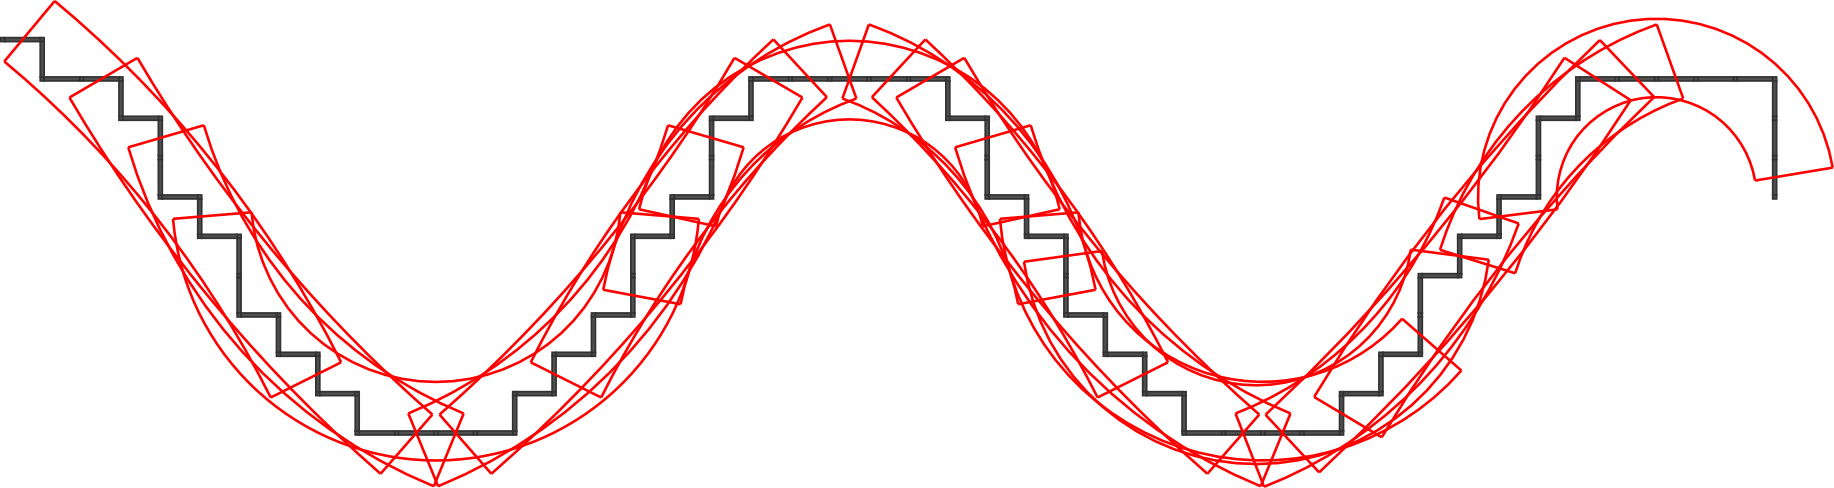
\includegraphics[width=13cm]{images/Notions/DCA2}
    \end{center}}
    \caption[Arcs de cercle digitaux reconnus.]{Arcs de cercle digitaux reconnus sur une forme de dimension 2.\label{fig:dca-figure2}}
\end{figure}


Nous verrons dans le chapitre suivant des estimateurs utilisant ces primitives
digitales pour estimer la courbure. Nous allons également proposer un estimateur
digital de courbure tirant parti des segments maximaux.
%\section{Enveloppes convexes}
%
\section{Conclusion}
%
Nous avons dans ce chapitre posé les bases de la géométrie différentielle et de
la géométrie digitale.  Ces bases vont nous permettre dans le chapitre suivant
de définir formellement des estimateurs digitaux de courbures en dimension 2 et
3. De plus, la reconnaissance de primitives nous permettra d'adapter nos
estimateurs en analysant au préalable la géométrie de la forme d'entrée.
